\chapter{Literature review}\label{ch:LiteratureReview}

\ifpdf
    \graphicspath{{Chapter2_LitReview/Chapter2Figs/PNG/}{Chapter2_LitReview/Chapter2Figs/PDF/}{Chapter2_LitReview/Chapter2Figs/}{Chapter2_LitReview/Chapter2Figs/Classification/}{Chapter2_LitReview/Chapter2Figs/Detection/}{Chapter2_LitReview/Chapter2Figs/Restoration}}
\else
    \graphicspath{{Chapter2_LitReview/Chapter2Figs/EPS/}{Chapter2_LitReview/Chapter2Figs/}}
\fi

The literature review presented in this chapter is split into three major sections: Classification, Detection and Restoration. These sections contain the literature review that forms the basis of each chapter of this thesis. The classification section covers literature reviewed for the work undertaken in chapters~\ref{ch:APR} and \ref{ch:MultichannelAPR} while the detection and restoration sections cover work undertaken in chapters~\ref{ch:TransientNoiseDetection} and \ref{ch:TransientNoiseRestoration}.

%Not JUST classification. Also some other stuff (needs to be removed)
\section{Classification}\label{sec:LitRev_Classification}
%\subsection{Computational auditory scene analysis (CASA)}
%The computational auditory scene analysis (CASA) approach to source separation attempts to mimic the auditory scene analyzing (ASA) capabilities of the brain by computational means. \cite{Wang2006} state: ``One may define the CASA problem as the challenge of constructing a machine learning system that achieves human performance in ASA''. In an attempt to make CASA systems more \emph{biologically relevant} many CASA systems limit their scope to either monaural or binaural input signals and hence replicating the ASA problem where only the signal from the two ears are present.
%
%More specifically CASA solutions aim to identify certain auditory object, such as characterizing note objects in terms of harmonicity, correlated modulation, duration of sinusoidal partials and common onset, and arranging these into streams using psycho-acoustic cues \citep{Ellis1996}. Proximity of time-frequency objects within the audio mixture can cause problems for CASA whereas ASA is able to retain a reasonable degree of separation of sources. These shortcomings of CASA have thus been the focus of much research. Examples of this is the integration of evidence derived from multiple grouping principles at several levels of abstraction \citep{Godsmark1999}, matching of timbre features learned on solo excerpts \citep{Kashino1998}, \citep{Kinoshita1999}, \citep{Eggink2003} (based on a Gaussian mixture model (GMM) classifier). More recently the overlap probability of frequency components has been introduced to improve algorithm performance \citep{Sakuraba2003}.
%
%CASA methods still suffer from a few drawbacks though. The brain's own ASA system is able to localize sources in a natural acoustic environment through what is known as the \emph{precedence effect}. In environments where a sound is reflected multiple times before reaching the listener, the brain is able to give \emph{precedence} to early arrival of sounds, such as the direct sound, and hence evaluate the true location of the sound. This precedence rule between grouping cues can be hard to assess \citep{Wang2006}, which is also why current methods are restricted to non-reverberant mixtures \citep{Vincent2006}.
%
%In the recent paper, \cite{Shao2010}, the authors present a CASA system for separating speech signals in the presence of other speech or noise. Their approach proceeds by tracking time-frequency units across time frames in 2 different stages. Firstly they use harmonicity to segregate the voiced portions of individual sources for each time frame using multipitch tracking. Secondly the time-frequency units are grouped across the time frames by utilizing knowledge from the speaker characteristics. The system proposed in \cite{Shao2010} mainly focusses on features such as onset/offset and periodicity which are not specific necessarily specific to the target source or even speech and as such this system works well for a variety of speech separation cases with a variety of noise scenarios.
%
%\subsection{Independent Component Analysis (ICA)}
%One of the most widely known and used methods for blind source separation (\gls{bss}) is independent component analysis (ICA). \gls{ica} proposes to separate a multivariate signals into additive subcomponents supposing the mutual statistical independence of the non-Gaussian source signals. For $M$ observations and $N$ sources it is a requirement for \gls{ica} to work that $M\geq N$.
%In general \gls{ica} can be defined as the linear transformation $\textrm{\textbf{A}}$ of observed data $\textrm{\textbf{x}} = [x_1,\ldots,x_M]$
%
%\begin{equation}\label{eq:ICA1}
%    \textrm{\textbf{x}} = \textrm{\textbf{A}}\textrm{\textbf{s}}
%\end{equation}
%
%where $\textrm{\textbf{s}}  = [s_1,\ldots,s_N]$ is the separated sources or components \citep{Virtanen2007}.
%
%Traditionally $\textrm{\textbf{A}}$ would then be referred to as the mixing matrix. The source signals $\textrm{\textbf{s}}$ can feasibly be recovered using $\textrm{\textbf{s}} = \textrm{\textbf{A}}^{-1}\textrm{\textbf{x}}$  with $\textrm{\textbf{A}}$ the invertible matrix.  $\textrm{\textbf{A}}^{-1}$ is then called the un-mixing matrix \citep{Smaragdis1998}.
%
%A very popular implementation of the \gls{ica} method is the FastICA algorithm as proposed in \cite{Hyvarinen1999}. Often mixture models are modeled as \emph{convolutive} and hence solving for the mixing matrix \textbf{A} in the time-domain will require labor-intensive convolution while some methods propose solutions to the inherent permutation problem for the frequency domain equivalent of the FastICA \citep{Mitianoudis2003}. It has been reported that this approach has also produced good separation results.
%
%A more recent paper \citep{Douglas2007} presents two spatio-temporal extensions to the FastICA method and reports significant improvements over previous methods when applied to multichannel recordings of two- and three-source speech mixtures in a room environment. It was also noted that this proposed method was simple, fast and did not require parameter tuning in order to obtain good separation performance.
%
%\subsubsection{Convolutive mixtures}
%Due to extensive filtering imposed upon real world signals by their environment and propagation delays, instantaneous mixtures are rarely encountered. Most real world mixtures tend to be of convolved mixtures \citep{Smaragdis1998}.
%
%Consider again the model from equation~(\ref{eq:ICA1}) but this time consider a mixture $\textrm{\textbf{x}}$ recorded in a real environment where the mixture can be approximated by a convolutive mixture of the source signals in the time domain,
%
%\begin{equation}\label{eq:ICA2}
%    \textrm{\textbf{x}}(t) = \textrm{\textbf{A}}(t) \ast\textrm{\textbf{s}}(t).
%\end{equation}
%
%Applying the Fourier transform (FT) yields:
%\begin{equation}\label{eq:ICA3}
%   \hat{ \textrm{\textbf{x}}}(\omega) = \hat{\textrm{\textbf{A}}}(\omega)\hat{\textrm{\textbf{s}}}(\omega),
%\end{equation}
%where $\hat{ \textrm{\textbf{x}}}(\omega), \hat{\textrm{\textbf{A}}}(\omega)$ and $\hat{\textrm{\textbf{s}}}(\omega)$ are the Fourier transform of $\textrm{\textbf{x}}(\omega), \textrm{\textbf{A}}(\omega)$ and $\textrm{\textbf{s}}(\omega)$ respectively \citep{Ikeda1999}.
%
%It is noted that if $\textrm{\textbf{A}}$ in equation~(\ref{eq:ICA1}) is seen as a matrix of \gls{fir} filters instead of scalars, the resulting multiplication will be equivalent to convolution and the notation will be consistent. This notation is called \gls{fir} algebra notation \citep{Lambert1996}.
%
%This time-frequency approach to ICA has been proposed by a variety of authors \citep{Lee1998}, \citep{Ikeda1999}, \citep{Smaragdis1998} and specifically \cite{Ikeda1999} has been successful in dealing with the inherent arbitrary scaling and permutation problems of the \gls{ica} approach applied in a frequency domain context \citep{Zhang2007}.
%
%The recent paper \cite{Zhang2007} attempts to avoid the whitening of outputs which plagues conventional implementations of \gls{ica} for convolutive mixtures by enforcing pairwise independence rather than mutual independence. This approach is based on the findings that for blind separation the two are generally equivalent.
%%better ending here?
%
%\subsection{Independent Subspace Analysis (ISA)}
%Independent subspace analysis (ISA) is based on \gls{ica} but relaxes the constraints $M\geq N$ and the statistical independence of source signals. In practice ISA is a generalization of \gls{ica} in the sense that instead of requiring statistical independence between components ISA requires statistical independence between groups of components. ISA can also been described as multidimensional independent component analysis and hence the independent components are required to be of the same dimension $k$. In the case where $k = 1$, ISA is equivalent to \gls{ica} \citep{Theis2006}. Despite this relaxing of restrictions of the \gls{ica} approach implementations of ISA has still been restricted by fixed group sizes or semi-parametric models. An even more general approach has been proposed which introduces the concept of irreducible independent components and give an identifiability result for this general, parameter-free model together with an arbitrary subspace size algorithm \citep{Theis2006}.
%
%A previous study managed to implement ISA models for audio source separation and introduced the \emph{ixegram} as a measure space for grouping independent basis components \citep{Casey2000}. The separation and grouping results from this experiment suggest that the technique can perform separation of source signals without parametric model fitting or prior knowledge of the composition of input data.
%
%\subsection{Non-Negative Matrix Factorisation (NMF)}
%Since the concept of non-negative matrix factorization (NMF) was introduced independently by \cite{Paatero1997} and \cite{Lee1999} the method has gained some popularity within the field of polyphonic transcription and the source separation field \citep{Smaragdis2003}, \citep{Smaragdis2004}. NMF was originally proposed as an alternative to $k$-means clustering and \gls{pca} for data analysis and compression.
%The original formulation of NMF starts with a non-negative $M\times N$ matrix $\textrm{\textbf{V}} \in \mathbb{R}^{\geq 0,M\times N}$ where the goal is to approximate $\textrm{\textbf{V}}$ as a product of two non-negative matrices so that
%
%\begin{equation}\label{eq:nmf1}
%    \textrm{\textbf{V}} \approx \textrm{\textbf{W}}\textrm{\textbf{H}}
%\end{equation}
%where $\textrm{\textbf{W}} \in \mathbb{R}^{\geq 0,M\times R}$, $\textrm{\textbf{H}} \in \mathbb{R}^{\geq 0,R\times N}$ and $R \leq M$ such that the error of reconstruction is minimized \citep{Smaragdis2004}.
%
%Good results have generally been reported for extraction of percussive sounds in mono recordings, but for low intensity sounds the algorithms generally perform worse and suffer from distortion and lost information inherent in the mixing and analysis process \citep{Smaragdis2004}. Other results have shown NMF to consistently obtain better separation results than ISA and \gls{ica} \citep{Virtanen2007}.
%
%\subsection{Hierarchical Bayesian Models}
%
%The task in Bayesian source separation is to infer $N$ source signals $s_{k,n} \equiv \textrm{\textbf{s}}$ given $M$ observed signals $x_{k,m} \equiv \textrm{\textbf{x}}$, where $n=[1,\ldots,N]$ and $m=[1,\ldots,M]$. Here $k=[1,\ldots,K]$ is an index which may correspond to time or to expansion coefficient of the sources in a linear transform domain. A Hierarchical Bayesian Model for the inference of the source signals can hence be formulated as
%
%\begin{equation}\label{eq:hbm1}
%    p(\textrm{\textbf{s}}|\textrm{\textbf{x}}) = \frac{1}{Z_x}\int p(\textrm{\textbf{x}}|\textrm{\textbf{s}},\Theta_m)p(\textrm{\textbf{s}}|\Theta_p)p(\Theta_p)p(\Theta_m)d\Theta_m d\Theta_p.
%\end{equation}
%
%Here the conditional distribution is characterized by the conditional distribution $p(\textrm{\textbf{x}}|\textrm{\textbf{s}},\Theta_m)$, where $\Theta_m$ denotes the collection of mixing parameters such as the mixing matrix, observation noise and variance, etc. and the prior term $p(\textrm{\textbf{s}}|\Theta_p)$ describes the sources via their own prior parameters $\Theta_p$ \citep{Cemgil2007}.
%
%It is worth noting that there is a considerable computational cost associated with a full Bayesian inference, via MCMC or variational Bayes (VB) for Bayesian source separation. Good results were reported in a study attempting Bayesian source separation using an MCMC approach to inference \citep{Fevotte2006}. Also, the authors of this study point out the computational burden of the MCMC approach compared to the alternative expectation maximisation (EM) approach. It was although also noticed that the \gls{em} approach was far more sensitive to mixing matrix initialization and hence less robust. The Gibbs sampler described in this paper was implemented as part of the review of this paper. Although the implementation was problematic due to the inherent indeterminacy on gain, the approach provided good results to noisy linear mixtures of sources.
%
%The recent paper \cite{Cemgil2007} describes a hybrid approach where a general linear instantaneous model, which might be noisy and underdetermined, is tackled using a Student $t$ distribution to model the source prior. Both the Gibbs sampler and VB method were studied as a method for inference. Both these methods are algorithmically similar but by employing a hybrid method the authors managed to combine the speed of the variational approach with the robustness of the Gibbs sampler \citep{Cemgil2007}.

\subsection{Audio classification}
This section contains a brief review of the methods typically employed in the field of audio classification. Classification features and classifiers are covered independently since, in many cases, they can be combined according to the particular application.

A variety of different features have been proposed for audio classification but features are mainly centered around the distinction between music, speech, silence and background noise. \gls{zcr} has been reported as a useful feature for a variety of audio signals although mainly used in speech/music classification algorithms \cite{Lu2002}. \gls{zcr} is defined as the number of time-domain zero-crossings within a given number of samples in the signal. Typically this number is divided by the number of samples within this frame. This feature is popularly used in music information retrieval and speech recognition \cite{Saraceno1997}\cite{Scheirer1997}\cite{Gouyon2000}. \gls{zcr} is also commonly used in \gls{vad} along with energy based detectors \cite{Sangwan2002}.

%SF (spectral flux)
\gls{sf} compares the power spectrum of neighbouring audio frames in an effort to measure how quickly the spectrum fluctuates. Typically this is done by calculating the Euclidian distance between two normalised spectral coefficients \cite{Wang2012}.
% \cite{Lu2001}\cite{Wang2012}

%NFR (Noise frame ratio)
The last audio feature presented here is the \gls{nfr} metric. This feature classifies frames as being noise frames if the local peak of their normalised correlation function reaches a certain threshold. The \gls{nfr} is then the ratio between noisy frames and non-noisy frames in the audio segment \cite{Lu2002}\cite{Jiang2000}.

%MFCC
\label{corrections:mfcc1}
Within the field of speech feature extraction the \gls{mfcc} is considered the most popular and has become the standard in speaker recognition systems partly due to its efficient computational scheme \cite{Tyagi2005}. The \gls{mfcc}s are obtained by mapping the power spectrum onto a Mel frequency scale using a series of triangular overlapping windows. The \gls{mfle} (log of the power) of each of the filters are calculated. The amplitude resulting from taking the \gls{dct} (or another linear transform) of the \gls{mfle}, as though it was a signal, will be the \gls{mfcc} \cite{Sahidullah2012}. In music genre classification \gls{mfcc} has also been used and it has been noted that specifically the lower \gls{mfcc}'s correlate well with the \emph{timbre} of the music \cite{Muller2010}. The \gls{mfcc} does although suffer from lack of robustness in the presence of common additive noise \cite{Tyagi2005}.

Many other features have been proposed and used successfully throughout the literature and an exhaustive list can be found here \cite{Scheirer1997} and \cite{Gouyon2000}.
%LSTER (low short-time energy ratio)
% \cite{Lu2001}

%KNN
% \cite{Lu2001}

%LSP VQ
% \cite{Lu2001}

In the area of audio classification a range of classifiers has been proposed. The most commonly used ones are discussed here.

The \gls{gmm} classifier assumes that each class pdf is comprised of a specific number of multidimensional Gaussian distributions. Iterative \gls{em} can then be used to estimate parameters of each Gaussian component and the mixture weights \cite{Tzanetakis2002}. \gls{k-nn} is a non-parametric classifier where samples are classified according to the majority of its K nearest neighbors \cite{Lu2001}. Both of these classifiers have performed similarly to humans in genre classification applications \cite{Tzanetakis2002} and in speech/music classification/segmentation applications \gls{k-nn} has given total accuracy rates over 96\% using a variety of features such as \gls{zcr}, \gls{sf} and \gls{nfr} among others \cite{Lu2002}. \gls{hmm} classifiers have also been employed where the \gls{hmm} is trained using \gls{ml} based on a training sequence \cite{Kimber1997}\cite{Xiong2003}\cite{Burke2013}. A classification algorithm employed in the context of \gls{hmm} was the Viterbi algorithm which is covered in more detail later in this chapter \cite{Kimber1997}\cite{Burke2013}.
A comprehensive introduction to various pattern recognition methods can be found in \cite{Duda2001}.

A study of 143 classification features for general audio data found that \gls{mfcc} and \gls{lpc} provided ``much better classification accuracy'' compared to spectral features \cite{Li2001}. This was concluded irrespective of the number of audio categories desired.
%hidden Markov model-based (\gls{hmm}-based) classifiers
% - http://www.sciencedirect.com/science/article/pii/S0167865500001197#BIB8
% - http://www.sciencedirect.com/science/article/pii/S0167865500001197#BIB9
%neural network-based classifiers http://www.sciencedirect.com/science/article/pii/S0167865500001197#BIB4
%decision trees, http://www.sciencedirect.com/science/article/pii/S0167865500001197#BIB8

\subsection{Principal component analysis (PCA)}
The central idea of \gls{pca} is to reduce the number of dimensions of a set of data consisting of potentially correlated variables to a smaller number of uncorrelated variables. This operation is achieved by transforming to a set of uncorrelated variables, principal components, which are ordered so the first principal component retains most of the variability and each succeeding component accounts for as much of the remaining variability as possible.

Take $\textrm{\textbf{x}}$ to be a vector of $p$ random variables where the variance of the variables and the correlation or covariance between them are of interest. The approach taken by \gls{pca} is to look for a few ($<<p$) derived variables which preserve most of the information given by these variances and covariances or correlations. The initial step is to look for a linear function $\boldsymbol\alpha_1^T \textrm{\textbf{x}}$ of $\textrm{\textbf{x}}$ which maximizes the variance, where $\boldsymbol\alpha_1^T =  [\alpha_{1{}1},\alpha_{1{}2},\ldots,\alpha_{1{}p}]$ so that:

\begin{equation}\label{eq:PCAdef}
\boldsymbol\alpha_1^T \textrm{\textbf{x}}= \alpha_{1{}1}x_1 +\alpha_{1{}1} x_2 + \ldots \alpha_{1{}p} x_p = \sum^p_{j=1}\alpha_{1{}j}x_j,
\end{equation}

is the first PC where ${}^T$ denotes a transposed matrix.
Now, find the linear function $\boldsymbol\alpha_2^T \textrm{\textbf{x}}$ of $\textrm{\textbf{x}}$ uncorrelated with $\boldsymbol\alpha_1^T \textrm{\textbf{x}}$ which again maximizes the variance, and so on, so that the $k$th PC $\boldsymbol\alpha_k^T \textrm{\textbf{x}}$ maximizes the variances while being uncorrelated to $\boldsymbol\alpha_1^T \textrm{\textbf{x}}, \boldsymbol\alpha_2^T \textrm{\textbf{x}}, \ldots, \boldsymbol\alpha_{k-1}^T \textrm{\textbf{x}}$. For a reduction of dimensionality it is hoped that most of the variability of $\textrm{\textbf{x}}$ is accounted for by $q$ principal components where $q<<p$ \citep[chap. 1]{Jolliffe1986}.

A more common transform into uncorrelated basis functions is the \gls{dft} or Fourier transform which approximately decomposes a signal into a set of uncorrelated or orthogonal (in the statistical sense) complex exponentials of the form $e^{i\omega t}$. The transform described above can therefore be seen as a generalization of the \gls{dft} for random processes, where the decomposed uncorrelated basis functions are real random signals rather than complex exponentials \citep[chap. 4.6]{Therrien1992}.

\subsection{Simple PCA Examples}

Figure~\ref{fig:30observations} gives a plot of 30 observations of two highly correlated (non zero mean) variables $x_1$ and $x_2$. It is seen that although there is considerable variation in the two variables, it is also noticed that there is more variation in the direction $x_2$.
\begin{figure}[!]
  \begin{center}
    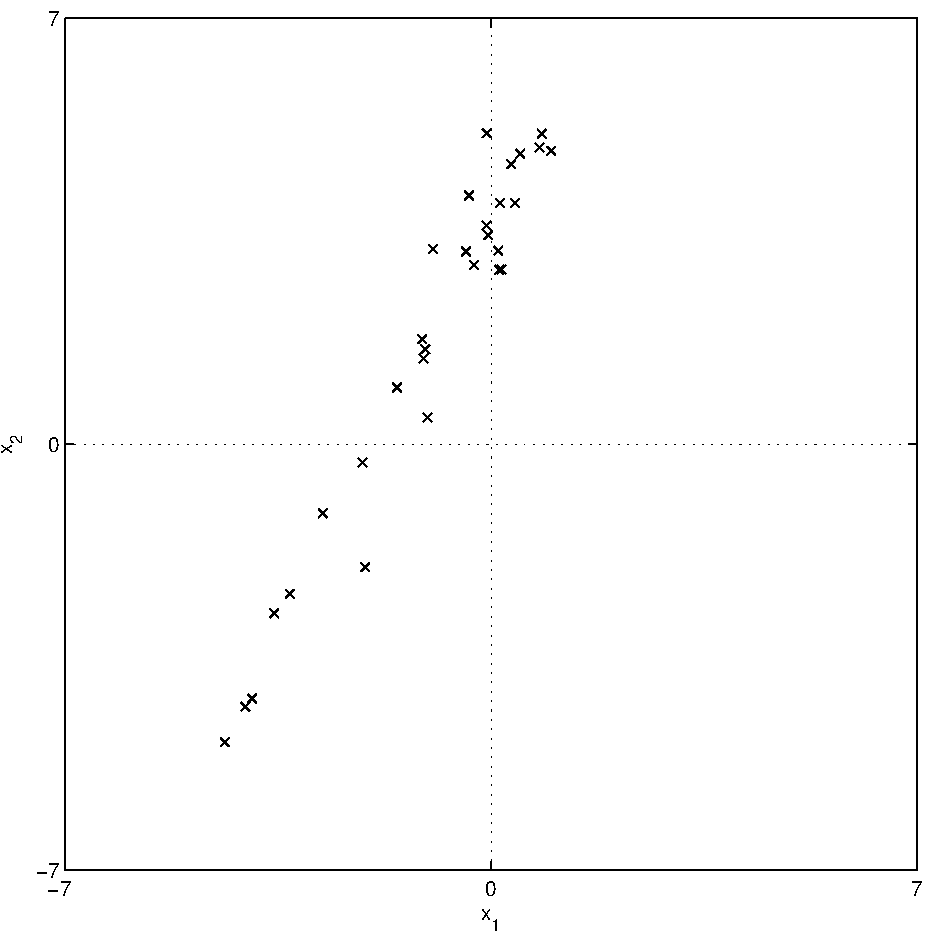
\includegraphics[width=260px]{30observations.pdf}
    \caption{Plot of 30 observations of variables $x_1$ and $x_2$.}\label{fig:30observations}
  \end{center}
\end{figure}

It is also seen in Figure~\ref{fig:30observations} that neither of the two variables have a mean of zero. To apply \gls{pca} the mean of both variables must be subtracted. Figure~\ref{fig:30observationsBar} shows the two variables with their means subtracted.
\begin{figure}[!]
  \begin{center}
    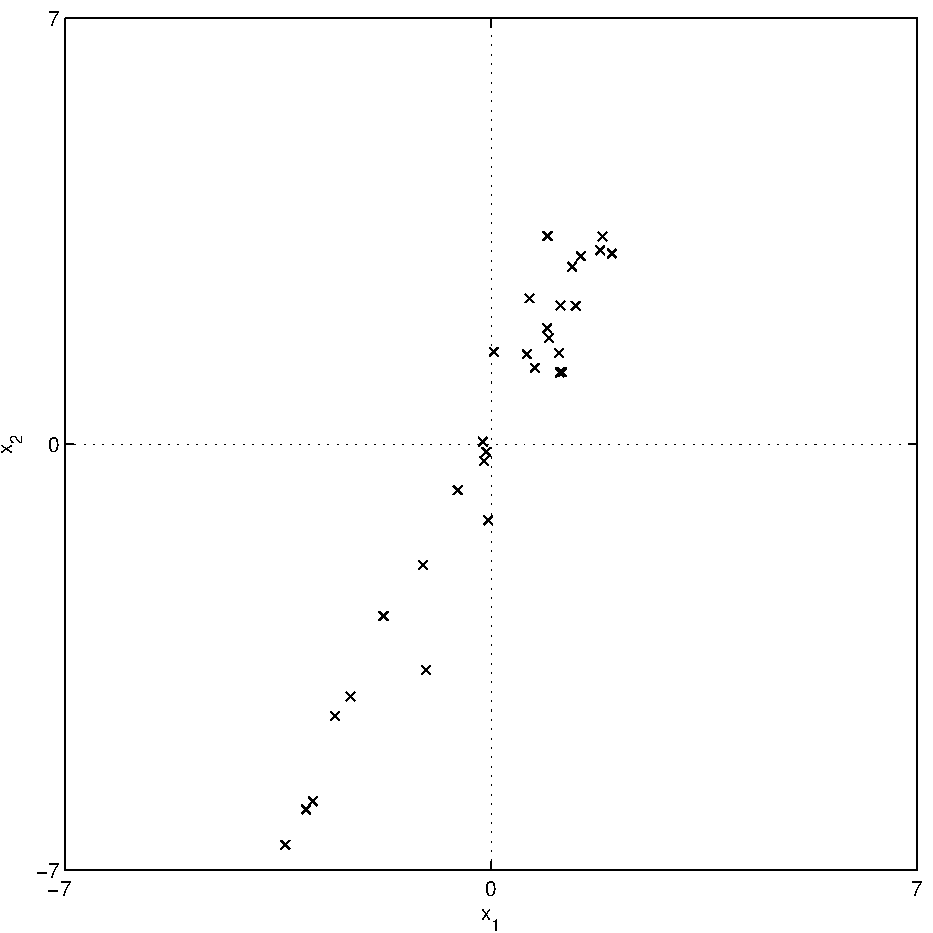
\includegraphics[width=260px]{30observationsBar.pdf}
    \caption{Plot of 30 observations of variables $x_1$ and $x_2$ with means subtracted.}\label{fig:30observationsBar}
  \end{center}
\end{figure}

Since the process of \gls{pca} is closely related to the diagonalization of the correlation matrix \citep[p. 174]{Therrien1992}, a helpful interpretation of the \gls{pca} is the attempt to ``rotate'' the axes of Figure~\ref{fig:30observationsBar} to collect as much variability as possible in one dimension, rather than having it spread over 2 dimensions. The correlation matrix (correlation coefficients) for the two variables $x_1$ and $x_2$ is,

\begin{equation}\label{eq:corrcoef}
\textrm{Correlation matrix} = \textrm{corr}(x,y)= \left(
    \begin{array}{cc}
        1   & 0.97 \\
        0.97& 1    \\
    \end{array}\right),
\end{equation}
where the correlated nature of the two variables is clearly seen by the almost unitary off-diagonal terms. Since the covariance matrix $\boldsymbol\Sigma$ is square it is possible to look at the eigenvalues and eigenvectors of it, which are,

\begin{eqnarray}\label{eq:eigValues}
\textrm{Eigenvalues} &=& \boldsymbol\lambda = \left(
    \begin{array}{c}
        \lambda_1 \\
        \lambda_2 \\
    \end{array}\right) = \left(
    \begin{array}{c}
        11.85 \\
        0.107 \\
    \end{array}\right)\\\label{eq:eigenVectors}
    \textrm{Eigenvectors} &=& \boldsymbol\alpha = \left( \boldsymbol\alpha_1 \quad \boldsymbol\alpha_2\right) =\left(
    \begin{array}{cc}
         0.451 & -0.892  \\
         0.892 & 0.451   \\
    \end{array}\right).
\end{eqnarray}

The eigenvectors from equation~(\ref{eq:eigenVectors}) have been plotted on top of the data in Figure~\ref{fig:30observationsBarEig}. These eigenvectors reveal information about patterns in the data, and as expected a clear correlation is found by the eigenvector $\boldsymbol\alpha_1$ between the variables $x_1$ and $x_2$. The second eigenvector $\boldsymbol\alpha_2$ gives the other, less important, pattern in the data.

\begin{figure}[!]
  \begin{center}
    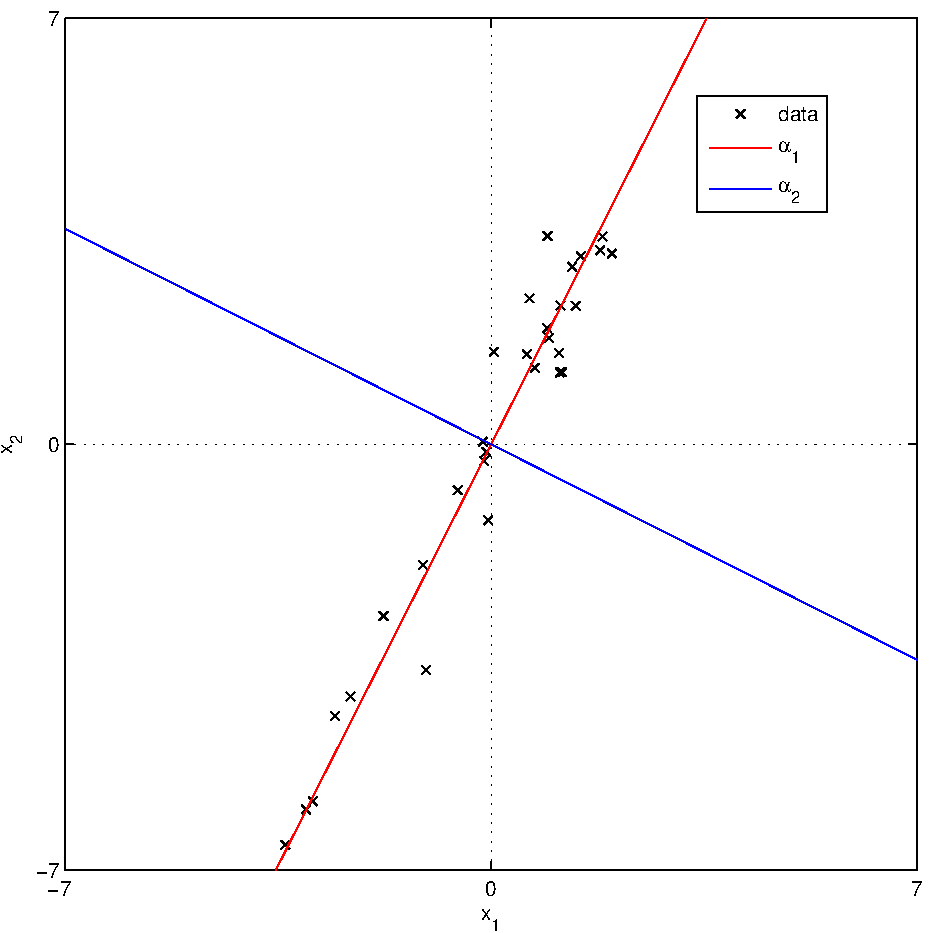
\includegraphics[width=260px]{30observationsBarEig.pdf}
    \caption{Plot of 30 observations of variables $x_1$ and $x_2$ with means subtracted, and eigenvectors of covariance matrix $\boldsymbol\Sigma$ plotted on top of the data. $\boldsymbol\alpha_k$ refers to the $k$th eigenvector.}\label{fig:30observationsBarEig}
  \end{center}
\end{figure}

The eigenvector with the highest corresponding eigenvalue is the first principal component. Ordering the eigenvectors in terms of descending eigenvalue gives the components in order of significance. It turns out that, for $k \in \{1, 2, \ldots, p\}$ the $k$th PC is given by $z_k = \boldsymbol\alpha_k^T\textrm{\textbf{x}}$, where $\textrm{\textbf{x}} = [x_1,x_2,\ldots, x_p]^T$ and where $\boldsymbol\alpha_k$ corresponds to the eigenvector with the $k$th largest eigenvalue \citep[p. 2-3]{Jolliffe1986}. For a complete transformation of the data use the expression $\textrm{\textbf{z}} = \hat{\boldsymbol\alpha}^T\textrm{\textbf{x}}$ where $\hat{\boldsymbol\alpha}$ is the feature vector containing the number of eigenvectors desired $q$, so $\hat{\boldsymbol\alpha} = [\boldsymbol\alpha_1,\boldsymbol\alpha_2,\ldots,\boldsymbol\alpha_q]$. Figure~\ref{fig:30observationsBarEig} shows the transformed data in terms of the transformed variables $z_1$ and $z_2$.

\begin{figure}[!]
  \begin{center}
    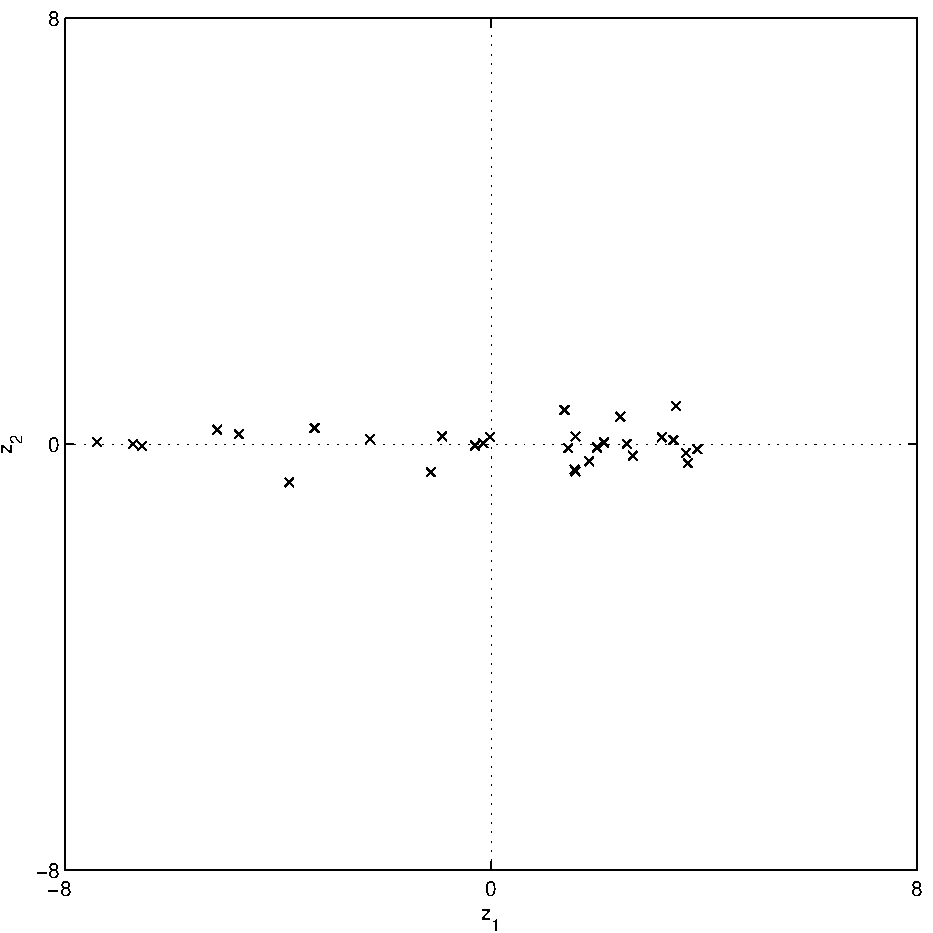
\includegraphics[width=260px]{30observationsBarTrans.pdf}
    \caption{Plot of 30 observations of variables $x_1$ and $x_2$ transformed into $z_1$ and $z_2$. Almost all the information or variability is now in $z_1$.}\label{fig:30observationsBarTrans}
  \end{center}
\end{figure}

It is noticed that this transform, with results displayed in Figure~\ref{fig:30observationsBarTrans}, does not actually reduce the dimensionality of the data since $q=p$ and hence all information is preserved. By making $q<p$ the dimensionality is reduced and less significant data is discarded. Since it is noticed from equation~(\ref{eq:eigValues}) that $\lambda_1$ is much larger than $\lambda_2$, and hence $\boldsymbol\alpha_1$ is a far more significant component in the data than $\boldsymbol\alpha_2$, one could feasibly define the feature vector as $\hat{\boldsymbol\alpha} = \boldsymbol\alpha_1$. Figure~\ref{fig:30observationsFinal} shows a transformation of the 30 observations for the scenario where $q=1$. The data has been transformed back into $x_1$ and $x_2$ and the original means of the data has been reapplied.

\begin{figure}[!]
  \begin{center}
    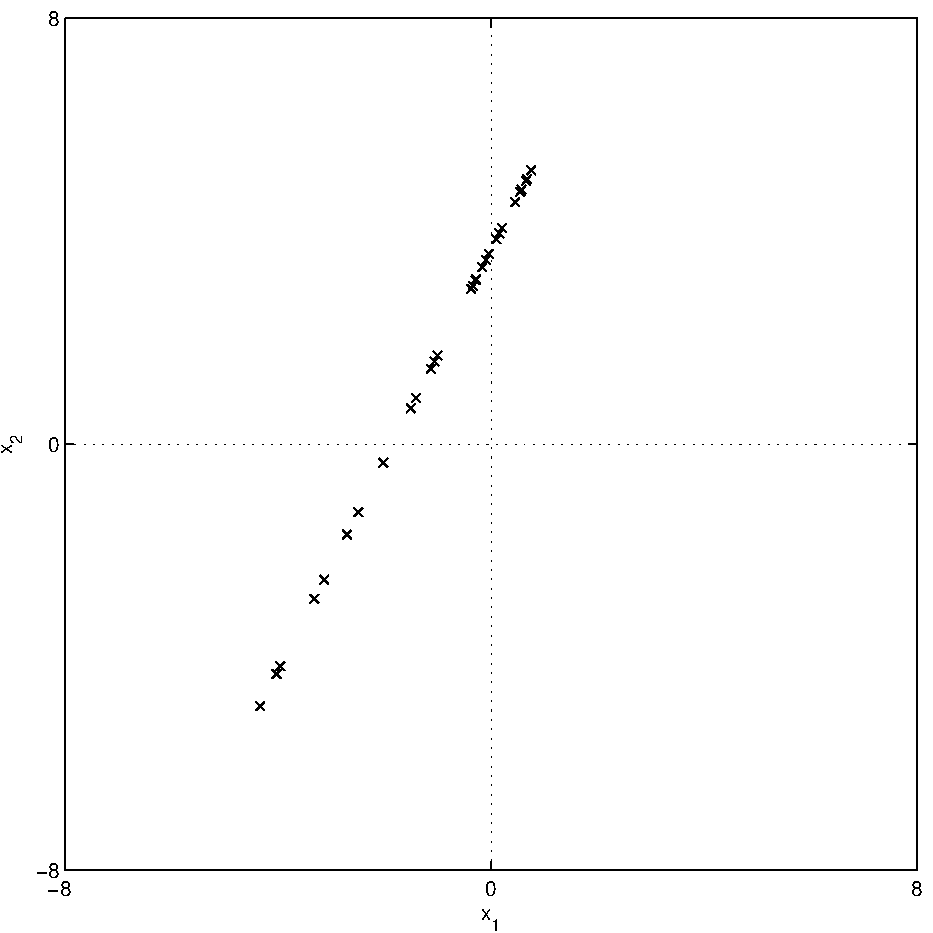
\includegraphics[width=270px]{30observationsFinal.pdf}
    \caption{Plot of 30 observations of variables $x_1$ and $x_2$ transformed from only $z_1$ with original means added back in.}\label{fig:30observationsFinal}
  \end{center}
\end{figure}

It is clear how the data resembles that of Figure~\ref{fig:30observations} although some of the variability has been lost in the dimensional reduction.

%\subsubsection{Eigenfaces}
%A popular application of \gls{pca} is the so called \emph{eigenfaces}\cite{Sirovich1987}\cite{Turk1991}\cite{Zaeri2006}. \emph{Eigenfaces} are essentially eigenvectors derived from the covariance matrix of a high dimensional vector space or ensemble of individual pictures. The idea of \emph{eigenpictures} was originally developed by \cite{Sirovich1987} were the authors repeatedly draw parallels between how humans recognize facial features and their own computational method. Although the \emph{eigenpictures} were not formerly used for facial recognition until \cite{Turk1991}, where the term \emph{eigenfaces} was first coined, \cite{Sirovich1987} hypothesises that perhaps humans compartmentalize faces and treat different features individually. This assertion is rooted first in the observation that humans are able to store and recognize enormous numbers of faces and secondly, that since recognition is apparently instantaneous it is conceivable that we do it by some efficient method, possibly similar to low dimensional methods. It is for example noted that ``(...) fewer than 100 \emph{eigenpictures} are necessary to fit a picture.'' and ``fewer than 100 dimensions are needed to provide likeness.''.
%
%The method used in \cite{Sirovich1987} uses photographs of 115 male undergraduates faces. These pictures were then digitized to a 128 by 128 pixel image and manually aligned. Figure~\ref{fig:Sirovich1987-3} shows a figure of 3 cropped images. The left image is the average face based on the ensemble, the middle is a sample face and right image that sample faces departure from the ensemble average or the samples \emph{caricature}. All pictures presented in this section are reproduced from the original paper \cite{Sirovich1987} where none of the pictures have been filtered to eliminate the high frequencies produced by digitization.
%
%\begin{figure}[!]
%  \begin{center}
%    \includegraphics[width=410px]{Sirovich1987-3.pdf}
%    \caption{Cropped faces: left, the average; middle, a sample face; right, its caricature.}\label{fig:Sirovich1987-3}
%  \end{center}
%\end{figure}
%
%The covariance matrix of the aligned ensemble is now calculated and all the \emph{eigenpictures} determined. Figure~\ref{fig:Sirovich1987-4} shows the first 8 of these \emph{eigenpictures} going from the top left frame, moving right and ending on the bottom right frame with the 8th \emph{eigenpicture}.
%
%\begin{figure}[!]
%  \begin{center}
%    \includegraphics[width=270px]{Sirovich1987-4.pdf}
%    \caption{First 8 \emph{eigenpictures} starting at upper left, moving to the right, and ending at lower right.}\label{fig:Sirovich1987-4}
%  \end{center}
%\end{figure}
%
%Figure~\ref{fig:Sirovich1987-5} shows the approximate reproduction of the sample face from Figure~\ref{fig:Sirovich1987-3} reproduced using 10, 20, 30 and 40 components.
%
%\begin{figure}[!]
%  \begin{center}
%    \includegraphics[width=270px]{Sirovich1987-5.pdf}
%    \caption{Approximation of the original picture (middle picture of Figure~\ref{fig:Sirovich1987-3}) using 10, 20, 30 and 40 \emph{eigenpictures}.}\label{fig:Sirovich1987-5}
%  \end{center}
%\end{figure}

\subsubsection{In the literature}
As mentioned previously, one of the main applications of \gls{pca} is dimensionality reduction which has rendered it useful in a variety of compression applications \citep{Vasilescu2003}\cite{Alexa2000}\linebreak[2]\cite{Zaeri2006}. Within the image compression community \citep{Vasilescu2003} the focus on principal components has been useful in dimensionality reduction, and more specifically it has been widely applied as a way of representing animations of 3D geometric shapes. \cite{Alexa2000} presented an ``easy and adaptive lossy compression'' algorithm which provided compression of animation sequences with a factor of 1:100 accepting loss in animation accuracy. Another approach to animation compression is presented in \cite{Karni2004} where \gls{pca} is combined with \gls{lpc} to individually focus on spatial and the resulting temporal components respectively.

PCA has been adopted as a way to manage the enormous amounts of data produced by microarray experiments in genetics \cite{Raychaudhuri2000}\cite{Saidi2004}. It was found that most of the observable variation in the data could be accounted for in just two components with rapidly falling eigenvalues \cite{Raychaudhuri2000}. In other words, \gls{pca} reduces the data to two data sets which capture most of the information \cite{Raychaudhuri2000}. Later research has highlighted some advantages in \gls{ica} over \gls{pca} for this application \cite{Saidi2004}. This approach has shown to be robust to significant noise levels, while \gls{ica} showed some domain specific feature extraction advantages.

The MPEG-7 standard \cite{Casey2001} has adopted a generalised sound recognition framework where decorrelated dimension-reduced features, called audio spectrum project (ASP), are used to train \gls{hmm} for classification \cite{Kim2006}. These features are regularly extracted from a basis decomposition via \gls{ica} or \gls{pca} \cite{Casey2001}\cite{Kim2003}\cite{Kim2006}. ASP features for sound recognition have been compared to \gls{mfcc} and were found to be slower and have worse performance \cite{Kim2004} while similar MPEG-7 related facial recognition tasks have yielded good performance but with a significant computational cost for the feature extraction step \cite{Zaeri2006}.
% \cite{Kim2003} %Speaker Recognition Using MPEG-7 Descriptors
% \cite{Zaeri2006} %Extension of the MPEG-7 Fourier Feature Descriptor for Face Recognition using PCA,
% \cite{Casey2001} % Basis functions may be chosen as uncorrelated features. (PCA or KL)

Although \gls{pca} is optimal in approximating the input data in the mean-squared error sense, the representation that it provides is often not the most meaningful in terms of real world data and in terms of describing the fundamental properties of the data. Since the \gls{pca} describes the data in an orthonormal basis, purely in order of the second-order statistics (covariance) of the input data \citep{Oja1995}, the \gls{pca} networks are only able to realize linear input-output mappings \citep{Karhunen1995}. In the field of neural networks there has been an interest in the development of nonlinear \gls{pca} methods that take higher-order statistics into account.

Although not specifically a \gls{pca} approach, \cite{Honkela2005} presents an approach to general nonlinear generative models for non-linear factor analysis which can form the basis for many non-linear implementations of latent variable models such as a non-linear generalization of \gls{pca} or even \gls{ica}. This general model is based on the variational Bayesian framework, which forms a solid foundation for non-linear modeling \citep{Honkela2005}. This model can be implemented into a linear \gls{ica} framework for nonlinear \gls{bss}, and \cite{Valpola2003} found that the variational Bayesian method provided ``useful'' results for difficult nonlinear problems. \citep{Lappalainen2000} introduced nonlinear counterparts of \gls{pca} and \gls{ica} where the generative mapping from sources to data is not restricted to being linear. Here this mapping is modeled by a \gls{mlp} network and the distributions of source signals are modeled by Gaussians. The general form of the models discussed in this paper are of the form:

\begin{equation}\label{eq:nonlinear}
\textbf{x}(t) = f\left(\textbf{s}(t)\right) + \textbf{n}\left(t\right),
\end{equation}

where $\textbf{x}(t)$ are the observations at time $t$, $\textbf{s}(t)$ are the sources, $\textbf{n}(t)$ the noise and $f()$ the function which maps the sources to the observation space. In \cite{Lappalainen2000} the authors compare their approach favorably to previously suggested models for representing data with nonlinear coordinate systems, and they especially focus on their methods applicability in high dimensional applications.

Very recent work has compared a range of multi-linear function factorisation techniques for feature extraction for classification applications \cite{Burke2013}. The comparison was performed on a variety of data types including speaker recognition from spoken vowels. The article confirms previously presented results and emphasises the advantage and simplicity of the factorisation techniques in question in relation to \gls{hmm}s and the associated training required. The authors found that \gls{cv} and \gls{pca} generally produced features with the greatest separability of the ones tested but neither reportedly performed well for the audio application. Specifically it was found in \cite{Burke2013} that the \gls{pca} produced features of poor separability somewhat in contrast to \cite{Raychaudhuri2000}. This could potentially be due to the stacking, or lack thereof, employed by the authors. It is also noted that while \gls{pca} features, per definition, are ordered according to ``principality'', \gls{cv} features require additional training \cite{Burke2013}.

\subsection{Probabilistic PCA (PPCA)}
One of the notable features of the above derived definition of the \gls{pca} is the lack of a probabilistic model for the observed data. \cite{Tipping1999} proposes a latent variable model for determining the principal axis of observed data which is closely related to factor analysis. This model utilizes a \gls{ml} estimator to estimate the parameters of the latent variable model. This model is commonly known as a factor analysis model where the relationship is linear:

\begin{equation}\label{eq:facAn}
\textrm{\textbf{t}} = \textrm{\textbf{W}}\textrm{\textbf{x}} + \boldsymbol\mu + \boldsymbol\epsilon,
\end{equation}

in which the $d$-dimensional observations vector \textbf{t} is related to a corresponding $q$-dimensional vector of latent (or unobserved) variables \textbf{x}. The $d \times q$ matrix \textbf{W} relates the two sets of variables, $\boldsymbol\epsilon$ is a zero-mean Gaussian noise process and the parameter $\boldsymbol\mu$ allows for the model to have a non-zero mean. By defining $\textrm{\textbf{x}} \sim \mathcal{N}_\textrm{x}(\boldsymbol0,\textrm{\textbf{I}})$ and $\boldsymbol\epsilon \stackrel{i.i.d.}{\sim} \mathcal{N}_\epsilon(\boldsymbol0,\boldsymbol\Psi)$, equation~(\ref{eq:facAn}) induces a Gaussian distribution for the observations $\textrm{\textbf{t}} \sim \mathcal{N}(\boldsymbol\mu,\textrm{\textbf{W}}\textrm{\textbf{W}}^T + \boldsymbol\Psi)$. The parameters of this model can then be obtained through an iterative process using \gls{ml} \citep{Tipping1999}.

 \cite{Lawrence2005} presents an extended \gls{ppca} model based on the work of \cite{Tipping1999} termed \gls{dppca}. The \gls{dppca} method can, through Gaussian processes, non-linearize the linear mappings from the embedded space and hence provide a new probabilistic approach to the visualizing and modeling of high dimensional data.



\section{Detection}\label{sec:LitRev_Detection}
Any restoration of transient noise events presupposes complete knowledge of the position of the corruption. In practice this information is unknown \emph{a priori} and a detection procedure must be employed to ascertain the timing of the corruptions. As noted in this section, a large number of different approaches to transient noise detection have been studied, and since there are as many types of transient noise as there are data that can be corrupted by it, the detection methods range from simple \emph{ad hoc} filtering approaches to more complex model based approaches.

In a reconstruction algorithm it is important to focus our attention on audible corruptions. The audibility of a corruption is not only a function of its amplitude or the energy that it represents, but also the context in which it sits. Psychoacoustically some corruptions may be rendered inaudible through masking effects such as the precedence effect, and hence any restoration effort is wasted or potentially damaging \cite{Moore2003}.

The simplest pulse detection algorithms exploit the relatively sparse nature of many audio, and in particular speech, signals above 9000 Hz in relation to impulsive noise which often exhibits much smoother and wider frequency characteristics \cite{Subramanya2007}. In \cite{Kasparis1993} and \cite{US6795559} the authors preprocess their signals using a high-pass filter to target the impulsive noise.

\subsection{Median filter methods}\label{sec:LitRevDetMedianFilts}
A classic pulse noise detection (and restoration) scheme involves a median filter \cite{Tukey1974}\linebreak[2]\cite{Lee1985}\cite{Heinonen1985}\cite{Heinonen1987}\cite{Maekivirta1991}\cite{Kasparis1993}.
%explain median filtering
Median filtering for signal smoothing, first published in \cite{Tukey1974}, has, according to \cite{Brillinger2002}, some important characteristics in that they reduce ``spiky'' noise while preserving jump discontinuities (edges). In \cite{Lee1985} it is noted that the median filter has limited effect on non-impulsive noise and the authors propose a method for augmenting the median filter with a linear filter for added smoothing. This augmentation of the nonlinear median filter approach with a linear filtering approach has become a popular variation of the median filtering process for impulsive noise detection and reduction, spawning a variety of implementations \cite{Lee1985}\cite{Heinonen1985}\cite{Nieminen1987}\cite{Kasparis1993}\cite{Loveridge1995}. In \cite{Kauppinen2002} it was also noted that the pulse detection algorithm that performed best was the median filter preprocessed by a linear filter. In recent years median based algorithms such as \gls{wm} filters \cite{Yin1996}\cite{Wang2010} and switching median filters \cite{Abreu1996}\cite{Chen2000}\cite{Chen2001}\cite{Lin2007} have seen a fair bit of attention although the focus of the implementations have almost exclusively been focused on image data.

The authors of \cite{Chandra1998} employ the \gls{sd-rom} (signal dependent rank order mean) algorithm, similar to the median filter methods, to evaluate the likelihood of each sample being corrupted based on the neighbouring samples. While this algorithm has shown great results in the removal of pulse noise in images \cite{Abreu1996}, in \cite{Chandra1998} the method performs best for short, although frequent, noise pulses of the order of a single or a few samples.

Since transient noise events often exhibit a sudden fast change in the signal, one way to detect the onset of a noise event is to detect abrupt nonstationary changes in the dynamics of time series. In \cite{Fancourt2000} the authors employ neural network predictors for this task, while \cite{Kauppinen2002} proposes an iterative discrete derivative method. In \cite{Kauppinen2002} the linear predictor and median hybrid method outperformed the derivative approach and the method described in \cite{Fancourt2000} was never tested on real data but the requirement for training and the inherent detection deadzone does reduce the method's general applicability.

\subsection{Autoregressive (AR) methods}\label{sec:LitRevAR}
While \gls{ar} methods have been used in other fields for detection and restoration of transient noise events \cite{Arakawa1986}, these methods were generally pioneered in the field of audio processing in \cite{Vaseghi1988thesis}\cite{Vaseghi1988}\cite{Vaseghi1990}. \gls{ar} methods are today the basis for many pulse detection algorithms in audio applications \cite{Karjalainen1997}\cite{Esquef2000}\cite{Haermae2000}\cite{Esquef2002}\cite{Kauppinen2002}\cite{Wolfe2005}\cite{Subramanya2007}. The \gls{ar} method considers a sub-frame of the audio data $x_t$ for $ t = \{ 1, \ldots, N \}$. Assuming the data is drawn from a short-term stationary \gls{ar} process:

\begin{equation}\label{eq:ARmodel}
x_t = \sum_{i=1}^P a_i x_{n-i} + ge_t,
\end{equation}

where $e_t$ is the prediction error (or excitation signal), $g$ is the excitation gain and $\mathbf{a} = \{a_1,\ldots,a_P\}$ is the \gls{ar} coefficients of order $P$. The transient nature of the impulsive noise pulses will most likely lead to very large prediction errors if an attempt is made to predict its value with previous values of $x_t$. It follows that if an inverse \gls{ar} filter is applied to an \gls{ar} signal segment corrupted with transient noise events, $y_t$ the prediction error $e_t = y_t - \sum_{i=1}^P a_i y_{n-i}$ is expected to be large when noise events are present while remaining low at other times \cite{Godsill1998book}.

In \cite{Vaseghi1990} the authors find that linear prediction systems, or \gls{ar} process, are ``adequate for modelling of speech signals whereas they can not model impulsive disturbances.''. This realisation is used to separate out the residual of the \gls{lpc} model effectively leaving the excitation noise in addition to the transient noise events, similarly to the preprocessing step of the favored approach in \cite{Kauppinen2002}.

A noisy speech signal $y_n$ can be modelled as an instantaneous mixture of a speech signal $x_n$ and some some impulsive disturbance:

\begin{equation}\label{eq:Vaseghi1990_1}
y_n = x_n + d_n,
\end{equation}

and assuming that the speech signal can be modelled with a linear prediction model,
\begin{equation}\label{eq:Vaseghi1990_4}
x_n = \sum^P_{k=1} a_k x_{n-k} +ge_n,
\end{equation}
where $\mathbf{a}$ contains the \gls{lpc} parameters, $e_n$ is the excitation signal and $g$ is the linear prediction system gain. The excitation signal can either be noise-like or a mixture of noise and some quasi periodic train of pulses. White noise can be considered as a basic excitation signal for speech modelling \cite{Vaseghi1990}.

Equation~\ref{eq:Vaseghi1990_1} can now be rewritten
\begin{equation}\label{eq:Vaseghi1990_5}
y_n = \sum^P_{k=1} a_k x_{n-k} + ge_n + d_n.
\end{equation}

With an estimate for the \gls{lpc} parameters $\mathbf{\hat{a}}$, the noisy signal $y_n$ can be written as the noisy excitation signal $v_n$

\begin{eqnarray}
% \nonumber to remove numbering (before each equation)
  v_n &=& y_n - \sum^P_{k=1} \hat{a}_k y_{n-k} \nonumber\\
  &=& x_n + d_h - \sum^P_{k=1} (a_k - \tilde{a}_k)(x_{n-k} + d_{n-k}),\label{eq:Vaseghi1990_6}
\end{eqnarray}

where $a_k$ is the error in the \gls{lpc} parameter vector estimate. Equation~\ref{eq:Vaseghi1990_6} can now be rewritten

\begin{equation}\label{eq:Vaseghi1990_7}
v_n = e_n + d_h - \sum^P_{k=1} \hat{a}_k d_{n-k} + \sum^P_{k=1} \tilde{a}_k x_{n-k}.
\end{equation}

The three elements that contribute to the noise in the excitation sequence estimate are the impulsive disturbance $d_n$, the past $p$ noise samples and the inflation in the variance of the residual signal due to the error parameter estimate \cite{Vaseghi1990}.
%\todo{maybe more sources for the separation?}

Since the transient noise pulses are transformed to a scaled version of the pulse response of the inverse \gls{lpc} filter, and experimental results conducted by \cite{Vaseghi1990} show the amplitude of the excitation signal is in the order of $10^{-1}$ to $10^{-4}$, the detection task is greatly simplified. The authors of \cite{Godsill1998} note that the disadvantages with the approach outlined in \cite{Vaseghi1990} is its inability to detect small pulses in the presence of much larger disturbances as well as the introduction of distortion for certain signals. In \cite{Godsill1998} the pulse detection problem is put in a Bayesian framework and extended to non-Gaussian noise pulses.

An adaptation to the basic \gls{ar} detection method in \cite{Vaseghi1988} uses a matched filter approach to detect transient noise events. The matched filter approach proceeds by considering the transient noise event as the signal and the \gls{ar} data as the coloured additive noise \cite{Godsill1998book}. An inherent problem with the matched filter approach is its dependence on training. Other methods in the literature model impulsive noise as non-Gaussian heavy-tailed distributions where the $\alpha$-stable distribution is particularly popular \cite{Tsihrintzis1997}\cite{Coates2002}. According to \cite{Nikias1995} $\alpha$-stable distributions are good for modeling many types of impulsive noise (including atmospheric and underwater acoustic noise). The sub-Gaussians methods in \cite{Tsihrintzis1997}\cite{Coates2002} appear to perform well on certain kinds of impulsive noise though it is questionable whether they could perform in a real time application with high pulse variability and high sample rates.

Figures~\ref{fig:LitRev_DetectCompare} and~\ref{fig:LitRev_DetectCompare2} compare the output of the 4 basic detection schemes discussed previously. The data presented in Figure~\ref{fig:LitRev_DetectCompare}(a) and Figure~\ref{fig:LitRev_DetectCompare2}(a) is speech data corrupted with keyboard tapping noise sampled at 44.1 kHz. Each primary tapping pulse has been marked as ``Ground Truth'' although secondary pulses can also be seen. Comparing the matched filter (b) and \gls{ar} prediction error (c) methods in Figures~\ref{fig:LitRev_DetectCompare} and~\ref{fig:LitRev_DetectCompare2} it is noted that the matched filter produces a more smeared response while, in some cases, picking out more subtle pulses \cite{Godsill1998book}, e.g. 3rd marked pulse in Figure~\ref{fig:LitRev_DetectCompare}. The median filtered (d) and the high pass-filtered (HP) (e) signals produce nearly identical results. These results are also superior in that they increase the margin between lowest correct detection and the highest false detection is larger than for the \gls{ar} prediction error (c) and potentially the matched filter (b). It is also noted that both the median and HP filtered signals pick up a faint secondary pulse just beyond the 6th confirmed pulse in Figure~\ref{fig:LitRev_DetectCompare}. For the matched filter (b) response this pulse is obscured due to temporal smearing. This secondary detection is typically associated with the lifting of a keyboard key and should therefore not be considered as a potential false detection. This and other intricacies of establishing a ground truth value for detections will be discussed in Chapters~\ref{ch:TransientNoiseDetection} and \ref{ch:TransientNoiseRestoration}.

\begin{figure}[!] %LitRev_DetectCompare
\centering
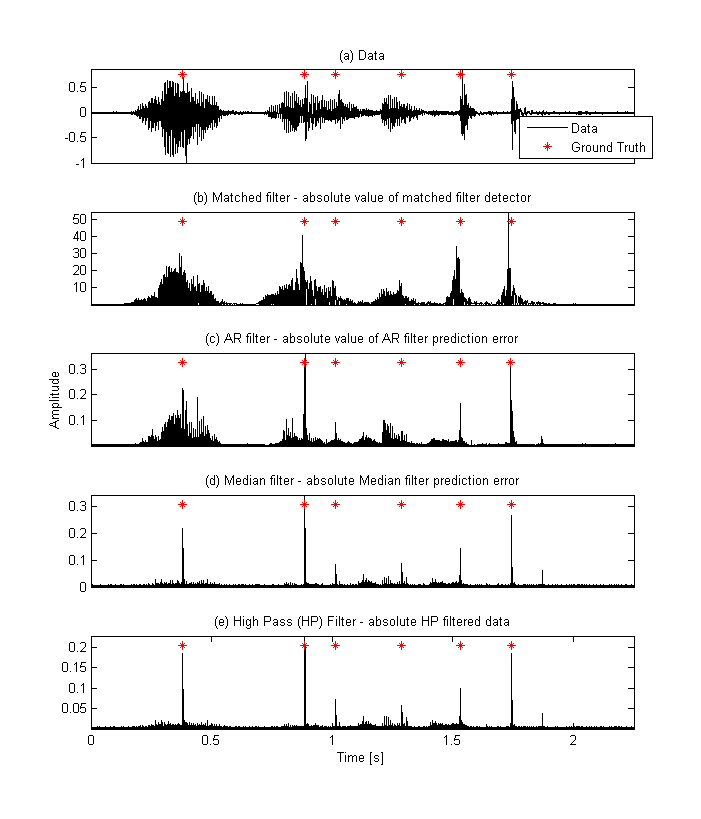
\includegraphics[width=130mm]{LitRev_DetectCompareNew.png}
\caption{Pulse detection comparison, (a) Speech data with 6 primary keystroke pulses sampled at 44.1 kHz, (b) absolute value matched filter detector output \cite{Vaseghi1988}, (c) absolute value of \gls{ar} filter prediction error output with buffer size 1024 samples and order 100 \cite{Vaseghi1990}, (d) absolute value of median filter prediction error \cite{Tukey1974}, and (e) absolute value of high pass filtered data with crossover frequency 9.6 kHz \cite{Godsill1998book}\cite{Kasparis1993}\cite{US6795559}.}
\label{fig:LitRev_DetectCompare}
\end{figure}

\begin{figure}[!] %LitRev_DetectCompare2
\centering
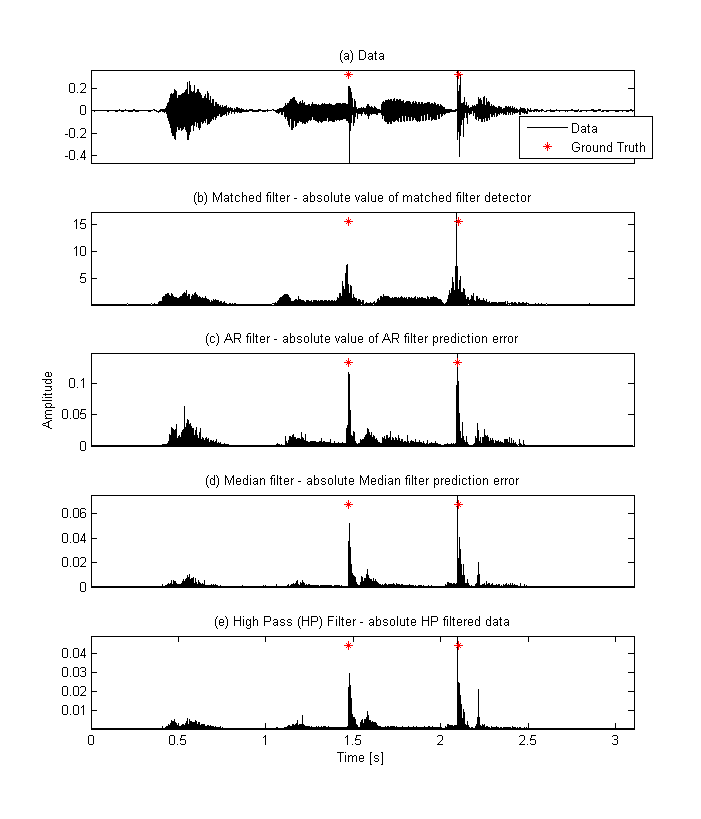
\includegraphics[width=130mm]{LitRev_DetectCompare2New.png}
\caption{Pulse detection comparison, (a) Speech data with 2 primary keystroke pulses sampled at 44.1 kHz, (b) absolute value matched filter detector output \cite{Vaseghi1988}, (c) absolute value of \gls{ar} filter prediction error output with buffer size 1024 samples and order 100 \cite{Vaseghi1990}, (d) absolute value of median filter prediction error \cite{Tukey1974}, and (e) absolute value of high pass filtered data with crossover frequency 9.6 kHz \cite{Godsill1998book}\cite{Kasparis1993}\cite{US6795559}.}
\label{fig:LitRev_DetectCompare2}
\end{figure}

%Warped linear prediction
\gls{wlp} is another adaptation of the \gls{ar} method \cite{Esquef2002}. The basic idea of \emph{warped} DSP was first introduced in \cite{Oppenheim1983} and later formalized in a predictive framework in \cite{Strube1980} and as a recursive filter \cite{Steiglitz1980}. \gls{wlp} has since been applied successfully to several audio applications \cite{Karjalainen1997}\cite{Haermae2000} and more specifically used as a basis for pulse detection \cite{Esquef2000}\cite{Esquef2002}.

The basic concept of warped filters can be explained by considering a standard \gls{fir}-like structure, but rather than applying the standard unit delay $z^{-1}$ the warped filter applies a new delay element $D(z)$ so that each new delay is frequency dependant (dispersive). In practice this means that the design of the warped filters are based on any pair of functions, $\tilde{z} = f(z)$ and $z = g(\tilde{z})$, so that $f(\cdot)$ and $g(\cdot)$ are one-to-one mappings of the unit circle onto itself, and $z = g\left( f(z) \right)$ \cite{Karjalainen1997}. Bilinear conformal mapping \cite{Brown1996} conforms to the requirements and corresponds to the first order all-pass filter

\begin{equation}\label{eq:Karjalainen1997}
\tilde{z}^{-1} = D(z) = \frac{z^{-1} - \lambda}{1 - \lambda z^{-1}},
\end{equation}

where $\lambda, -1 < \lambda < 1$, is a warping parameter which, if chosen appropriately \cite{Karjalainen1997}, yields a good match to the psychoacoustic Bark scale \cite{Smith1995}.

Warped digital filters have a range of advantages in that they can be designed to model the human auditory system as well as other physical systems \cite{Karjalainen1997}. In \cite{Esquef2002} the authors note that for auditory models the warping factor $\lambda$ tends to be positive while for click detection, negative warping factors appeared to perform best. It is also noted that pulse detection using \gls{wlp} comes at a considerable computational cost and is therefore not suited for real time implementations. As in \cite{Godsill1998book} the authors of \cite{Esquef2002} only considered pulses with duration of $<1$ ms, for which the \gls{wlp} based method performs well. This good performance is largely believed to be caused by spectral characteristics also exploited in \cite{Kasparis1993}\cite{US6795559}, although the signals in \cite{Esquef2002} were not exclusively corrupted speech data and can therefore not be assumed to be spectrally sparse at high frequencies.


%|P. A. A. Esquef, V. Välimäki, K. Roth, and I. Kauppinen, "Interpolation of Long Gaps in Audio Signals Using the Warped Burg's Method", in Proc. 6th Int. Conf. Digital Audio Effects %(DAFx-03), pp. 18-23 London, UK, September 8-11, 2003.

Warped-based methods evaluated via objective measures have been found to only be advantageous for lower model orders. For moderate model orders warped-based methods perform similarly to conventional schemes \cite{Esquef2003}\cite{Esquef2003a}. Furthermore it is reported that warped-based methods increase the number of floating-point operations by around 77\% \cite{Esquef2003}.

\subsection{Frequency methods}
 Some authors have attempted to use the \gls{stft} as a basis for detection \cite{Czyzewski1995}\cite{Subramanya2007}\cite{Sugiyama2007}\cite{Abramson2007} causing problems such as loss of temporal resolution of detections at moderate frame sizes, loss of spectral resolution for smaller frame size and computational inefficiency using extensive overlapping of frames. The authors of \cite{Subramanya2007} propose an algorithm for detection of keystroke noise on laptop computers and recognise the temporal and spectral variability in the noise pulses cause methods based on noise models and stationarity assumptions to perform poorly. Instead the authors propose to exploit the ``smoothness in speech signals present across time'' and the relative spectral sparsity of speech signals compared to keystroke noise pulses with a simple linear predictive model across each frequency bin. Their model assumes that

\begin{equation}
\label{eq:Subramanya2007}
S(k,t) = \sum_{m=1}^M \alpha_{km} S(k,t - \tau_m) + V(k,t),
\end{equation}

where, $S(k,t)$ represents the time-frequency component for $k$ and $t$, spectral and time index respectively, $\boldsymbol{\tau} = \left\{\tau_1, \ldots ,\tau_M \right\}$ defines the frames used, \linebreak[2]$\boldsymbol{\alpha}_k = \left\{\alpha_{k1},\ldots,\alpha_{kM} \right\}$ defines the weights used for the linear prediction, and $V(t,k)$ is some zero-mean Gaussian noise with variance $\sigma^2_{tk}$.

The authors of \cite{Subramanya2007} proceed to calculate the joint probability assuming independent frequency frames and eventually the log-likelihood $F_t$ will be

\begin{equation}
\label{eq:Subramanya2007_2}
F_t = - \frac{1}{2} \sum_k \frac{1}{\sigma^2_{tk}} \left( S\left(k,t\right) - \sum_{m=1}^M \alpha_{km} S(k,t-\tau_m)\right)^2 + C_{tk}
\end{equation}

where $C_{tk}$ is a constant.

\subsection{Hidden Markov models (HMM)}
While some detection algorithms quite simply base detections on magnitudes of some parameter \cite{Subramanya2007}\cite{Sugiyama2007}, in some situations it may be advantageous to attempt to model, probabilistically, the evolution of a sequence of hidden states. For this application the hidden \gls{hmm} is considered effective \cite{Rabiner1989}\cite{Xu2005}.

It is beyond the scope of this work to give a comprehensive introduction to \gls{hmm}s but \cite{Rabiner1989} provides a comprehensive introduction to \gls{hmm} in the field of speech processing.

%Viterbi
The Viterbi algorithm, first proposed in 1967 \cite{Viterbi1967} and originally developed as a method for decoding convolutional codes
from language identification \cite{Nagarajan2004}, is a recursive optimal solution to the problem of estimating the state sequence of a discrete-time finite-state Markov process \cite{Forney1973}. The Viterbi algorithm is therefore not a classification algorithm in the traditional sense but if you consider states as classes and each time step as correlated trials then the Viterbi algorithm does apply.\label{corrections:viterbi}

Given an observation of a sequence $y \in \{y_1,\ldots,y_K\}$ the Viterbi algorithm's goal is to find the most probable sequence of states $S \in \{S_0,\ldots,S_K \}$ given these observations assuming the successive Markov state probabilities $Pr(S_{k-1} \rightarrow S_{k})$ as well as the output probabilities $p(y_k | S_{k-1} \rightarrow S_{k})$ are mutually independent for $k$. The likelihood function for the path from $k=1$ to $k=K$ is given by

\begin{equation}\label{eq:viterbiLitRev}
L = \prod_{k=1}^K Pr(S_{k-1} \rightarrow S_{k}) p(y_k | S_{k-1} \rightarrow S_{k}).
\end{equation}

Typically the logarithm is here considered due to computational efficiency.

\begin{equation}\label{eq:viterbiLitRev2}
\log{\left(L\right)} = \sum_{k=1}^K m(y_k ; S_{k-1}, S_{k}),
\end{equation}

where $m$ is the \emph{branch metric} between two states $S_{k-1}, S_{k}$ defined as

\begin{equation}\label{eq:viterbiLitRev3}
m(y_k ; S_{k-1}, S_{k}) = \log{\left( Pr(S_{k-1} \rightarrow S_{k}) \right)} + \log{\left( p(y_k | S_{k-1} \rightarrow S_{k}) \right)}.
\end{equation}

The maximum \emph{state metric} $M_K(S^i)$ over all paths leading from the origin to the $i$th state and $K$th node $S_K^i$ is defined as

\begin{equation}\label{eq:viterbiLitRev4}
M_K(S^i) = \max \left( \sum_{k=1}^{k-1} m(y_k ; S_{k-1}, S_{k}) + m(y_K ; S_{K-1}, S_{K}^i)\right),
\end{equation}

for all paths $S_0,\ldots, S_{K-1}$.
To maximize this sum simply maximize the first $K-1$ terms for each state $S^j_{K-1}$ at the (K-1)th node, and then maximize the sum of this and the $K$th term over all states $S_{K-1}$. In other words:

\begin{eqnarray}\label{eq:viterbiLitRev5}
M_K(S^i) &=& \max \left( M_{K-1}(S^i) + m(y_K ; S_{K-1}^j, S_{K}^i)\right), \\ \nonumber
& & S_{K-1}^j,
\end{eqnarray}
which is the expression at the heart of the Viterbi algorithm \cite{Viterbi2006}.

%\todo{Add information about the \gls{hmm} and Viterbi in particular}
% \cite{Rabiner1989}\cite{Viterbi1967}\cite{Forney1973}

\subsubsection{Time-Frequency processing}
%The basics of time-frequency processing is the correlation of a .... %Simon made a mark over "is" in this sentence
Since the object of interest in our detection efforts is inherently transient and therefore localised in time, classic Fourier analysis has a significant shortcoming in that it provides no temporal information. The basis of time-frequency processing is the correlation of a signal with a family of waveforms that are well concentrated in time as well as in frequency \cite{Mallat1999} also called \emph{time-frequency atoms}\cite{Gabor1946}. The popular \gls{stft} used in numerous applications dates back to 1946 and the introduction of the windowed Fourier atoms to measure the ``frequency variations'' of sound. Given the real and symmetric window

\begin{equation}\label{eq:Mallat1999}
g_{u,\xi}(t) = \mathrm{e}^{i\xi t}g(t-u),
\end{equation}
where $\xi$ is a modulation frequency and $u$ is a translation, $g$ is normalized, $\|g\| = 1$, so that $\|g_{u,\xi}\| = 1$ for any $(u, \xi) \in \mathbb{R}^2$. The resulting windowed Fourier transform of $f \in \mathbf{L^2}(\mathbb{R})$ is

\begin{equation}\label{eq:Mallat1999_2}
S f(u, \xi) = \langle f, g_{u,\xi} \rangle = \int^{+\infty}_{-\infty}  f(t)g(t-u)\mathrm{e}^{-i\xi t} dt,
\end{equation}
which is also called the \gls{stft} since the window $g(t-u)$ has the effect of localising the Fourier integral in the region of $t=u$. $\mathbf{L^2}(\mathbb{R})$ describes finite energy functions $\int |f(t)|^2 dt < + \infty$.

To evaluate the energy density $P_S$ of the \gls{stft}, also called the \emph{spectrogram}, the squared magnitude is computed:

\begin{equation}\label{eq:Mallat1999_3}
P_S f(u,\xi) = |S f(u,\xi)|^2 = \left| \int^{+\infty}_{-\infty} f(t)g(t-u)\mathrm{e}^{-i\xi t} dt \right|^2.
\end{equation}

The \emph{spectrogram} of $f$ is a measure of the energy in the time-frequency neighborhood of $(u,\xi)$. This is also called the Heisenberg box of $g_{u,\xi}$ and is defined as a region in the time-frequency plane $(t, \omega)$ whose location and width depends entirely on the time-frequency spread of the window $g_{u,\xi}$ centered around $(u,\xi)$ \cite{Mallat1999}. For more details on the derivation of the time-frequency resolution of the windowed Fourier transform see Appendix~\ref{ap:TimeFreqResolutionFourier} on page~\pageref{ap:TimeFreqResolutionFourier}.

For the windowed Fourier transform the time spread $\sigma_t$ and frequency spread $\sigma_w$ are independent of $u$ and $\xi$. Therefore $g_{u,\xi}$ corresponds to a Heisenberg box of area $\sigma_t \sigma_\omega$ centered at $(u,\xi)$ as seen in Figure~\ref{fig:LitRev_HeisenbergBox_STFT}\cite{Heisenberg1927}. The size of the box is constant and therefore independent of $(u,\xi)$ meaning that the windowed Fourier transform has the same temporal and frequency resolution throughout the time-frequency plane \cite{Mallat1999}.

\begin{figure}[!] %LitRev_HeisenbergBox_STFT
\centering
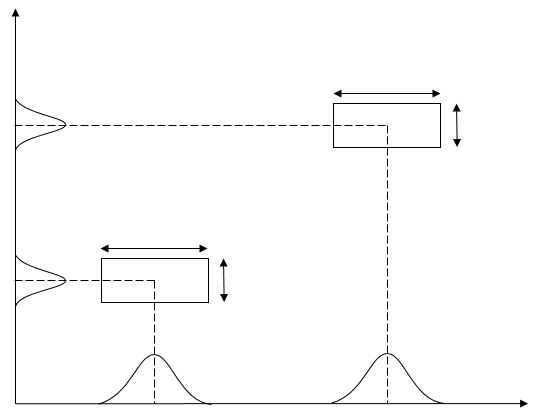
\includegraphics[width=80mm]{LitRev_HeisenbergBox_STFT_2.png}
\begin{picture}(0,0)
\put(-235,170){$\omega$}
\put(-235,122){$\gamma$}
\put(-235,55){$\xi$}
\put(-232,0){0}
\put(-169,-4){$u$}
\put(-67,-4){$v$}
\put(-7,2){$t$}

\put(-220,137){$|\hat{g}_{v,\gamma}(\omega)|$}
\put(-220,35){$|\hat{g}_{u,\xi}(\omega)|$}

\put(-169,75){$\sigma_t$}
\put(-133,57){$\sigma_\omega$}
\put(-150,20){$|g_{u,\xi}(t)|$}

\put(-70,142){$\sigma_t$}
\put(-32,122){$\sigma_\omega$}
\put(-50,20){$|g_{v,\xi}(t)|$}
\end{picture}
\caption{An example of the Heisenberg box illustration and the inherent time-frequency resolution trade-off for the \gls{stft}.}
\label{fig:LitRev_HeisenbergBox_STFT}
\end{figure}

In practice this gives rise to a trade-off between temporal and frequency resolution, illustrated in Figure~\ref{fig:LitRev_STFTlims}, where two different temporal frame sizes are shown in relation to the resulting frequency resolution.

\subsubsection{Wavelet decomposition}
The Wavelet Transform can be seen as a generalization of the windowed Fourier transform in that it decomposes a signal over dilated and translated wavelets. A wavelet is simply a function $\phi \in \mathbf{L^2}(\mathbb{R})$ which is normalised $\| \psi \| = 1$, centered in the neighborhood of $t=0$, and with zero average:

\begin{equation}\label{eq:Mallat1999_4}
\int^{+\infty}_{-\infty} \psi(t) dt = 0.
\end{equation}

Unlike the windowed Fourier transform the family of time-frequency wavelet atoms is translated by $u$ as well as scaled by $s$:

\begin{equation}\label{eq:Mallat1999_5}
\psi_{i,s}(t) = \frac{1}{\sqrt{s}}\psi\left(\frac{t-u}{s}\right).
\end{equation}

Now we have that the wavelet transform of $f \in \mathbf{L^2}(\mathbb{R})$ at time $u$ and scale $s$ is

\begin{equation}\label{eq:Mallat1999_x}
W f(u,s) = \langle f, \psi_{u,s} \rangle = \int^{+\infty}_{-\infty} f(t) \frac{1}{\sqrt{s}}\psi^\ast \left( \frac{t-u}{s} \right) dt.
\end{equation}

The energy spread of a wavelet time-frequency atom $\psi_{u,s}$ corresponds to a Heisenberg box centered at $(u,\eta/s)$ where $\eta$ is the center frequency of $\hat{\psi}$ the Fourier transform of $\phi$, and $\hat{\psi}_{u,s}$ is the Fourier transform of $\phi$ dilated by $1/s$. For more details on the derivation of the time-frequency resolution of the wavelet transform see Appendix~\ref{ap:TimeFreqResolutionWavelet} on page~\pageref{ap:TimeFreqResolutionWavelet}. The Heisenberg box remains of area $\sigma_t \sigma_\omega$ at all scales but it is now $s\sigma_t$ on the time axis and $\sigma_\omega /s$ along the frequency axis \cite{Mallat1999}. The temporal and frequency resolution is now dependent on $s$ as illustrated in Figure~\ref{fig:LitRev_HeisenbergBox_wavelets}

\begin{figure}[!] %LitRev_HeisenbergBox_wavelets
\centering
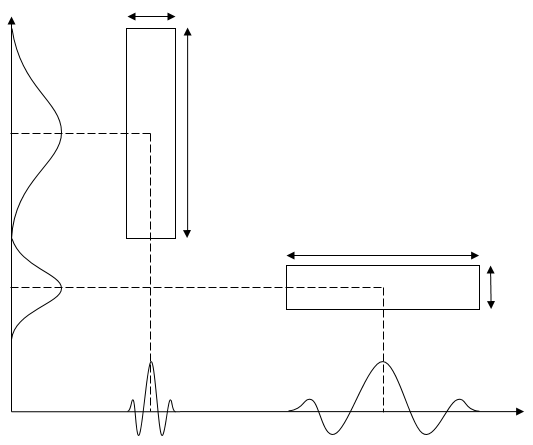
\includegraphics[width=80mm]{LitRev_HeisenbergBox_wavelets_2.png}
\begin{picture}(0,0)
\put(-235,180){$\omega$}
\put(-235,132){$\gamma$}
\put(-235,65){$\xi$}
\put(-232,10){0}
\put(-169,-4){$u$}
\put(-70,-4){$v$}
\put(-7,10){$t$}

\put(-220,140){$|\hat{g}_{v,\gamma}(\omega)|$}
\put(-220,75){$|\hat{g}_{u,\xi}(\omega)|$}

\put(-171,187){$\sigma_t$}
\put(-147,132){$\sigma_\omega$}
\put(-157,30){$|g_{u,\xi}(t)|$}

\put(-70,85){$\sigma_t$}
\put(-18,65){$\sigma_\omega$}
\put(-50,30){$|g_{v,\xi}(t)|$}
\end{picture}
\caption{The Heisenberg boxes for the wavelet transform.}
\label{fig:LitRev_HeisenbergBox_wavelets}
\end{figure}
The main difference between classic Fourier analysis and Wavelet analysis is that Wavelets are localised in both frequency and time whereas the Fourier transform is only localised in frequency. This leads to some significant advantages when considering data that is inherently transient. While the \gls{stft} does, to an extent, mimic the time localisation of the Wavelet Transform it does so at the cost of temporal resolution \cite{Mallat1999}. The trade-off between temporal and frequency resolution is illustrated in Figure~\ref{fig:LitRev_STFTlims} where two different temporal frame sizes are shown in relation to the resulting frequency resolution.

%LitRev_STFTlims
\begin{figure}
\centering
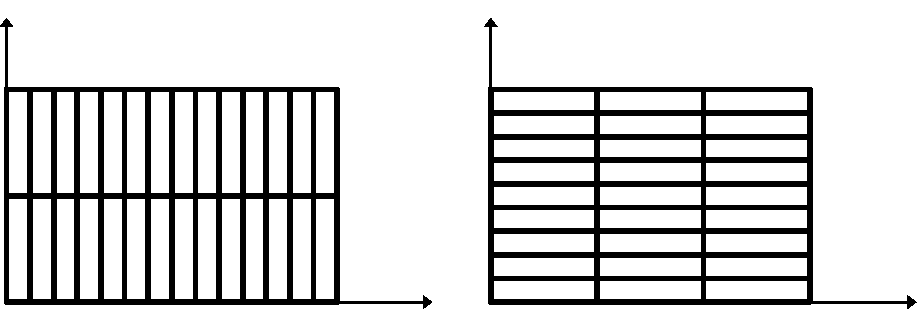
\includegraphics[width=120mm]{LitRev_STFTlims.pdf}
\begin{picture}(0,0)
\put(-355,120){Frequency}
\put(-200,0){Time}
\put(-175,120){Frequency}
\put(-20,00){Time}
\end{picture}
\caption{Heisenberg boxes of two wavelets. At larger scales the frequency resolution is increased by a decreased frequency support and the time spread is increased.}
\label{fig:LitRev_STFTlims}
\end{figure}

%LitRev_Wavelets
\begin{figure}
\centering
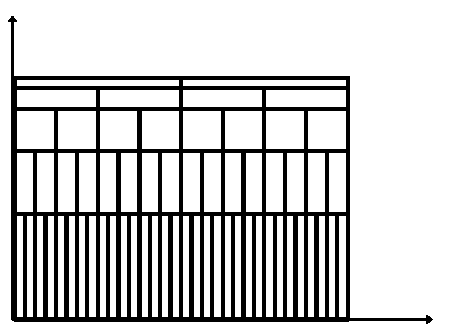
\includegraphics[width=65mm]{LitRev_Wavelets.pdf}
\begin{picture}(0,0)
\put(-195,133){Scale}
\put(-22,-7){Time}
\end{picture}
\caption{The scale-time relationship for the wavelet transform.}
\label{fig:LitRev_Wavelets}
\end{figure}

Figure~\ref{fig:LitRev_Wavelets} shows a similar plot to Figure~\ref{fig:LitRev_STFTlims} but for the Wavelet transform instead. It should be noted that a Wavelet spectrum, equivalent to a traditional spectrogram, is traditionally plotted in the time-scale space, where scale can be seen as being inversely proportional to frequency.

\subsubsection{Multi-resolution analysis with Filter Banks}
Consider now the discrete power spectral density calculation, from Equation~\ref{eq:Mallat1999_3}, for the signal $x(n)$:

\begin{equation}\label{eq:LitRev_Detection_PSD1}
S_{xx}(\omega) = \frac{1}{N} \left| \sum^{N}_{n=1} x(n) e^{-i \omega n} \right|^2.
\end{equation}

For a given frequency $\omega_i$, equation~\ref{eq:LitRev_Detection_PSD1} can be rewritten as

\begin{equation}\label{eq:LitRev_Detection_PSD2}
S_{xx}(\omega_i) = \left\| \sum^{N}_{k=1} h_i(k) x(n-k) \right\|^2,
\end{equation}

where

\begin{equation}\label{eq:LitRev_Detection_PSD3}
h_i(k) = w(k)e^{-i \omega_i n},
\end{equation}

and $w(k)$ is a window function. Considering $w(k)$ as a prototypical \gls{fir} lowpass filter, the collection of all $h_i(k)$s constitutes a bank of bandpass filters each centered on frequency $\omega_i$ \cite{Ariananda2013}. This implementation is commonly referred to as the periodogram but it also highlights what is sometimes called the filter bank paradigm and is a particularly simple implementation of the \gls{dwt}\cite{Mallat1999}.

Considering again the window function $w(k)$ from equation~\ref{eq:LitRev_Detection_PSD3}, the simplest window conceivable would be a simple rectangular window $w(k) = 1/N$. Naturally this would lead to significant side lobe leaks in the spectral domain and is therefore highly undesirable. Employing Hamming and Hann windows is a common approach to alleviate these issues. Another issue that arises with the periodogram is that its estimates are coarse with low precision and large variance \cite{Ariananda2013}. A common method for alleviating this variance problem is by windowing the data first \cite{Lim1988book}.

Work done on Multi Taper Spectrum Estimation (MTSE) \cite{Thomson1982} and later on multi-resolution theory \cite{Mallat1989}\cite{Meyer1995} proves that a conjugate mirror filter characterises a wavelet and that cascading these filters leads to a fast implementation of the discrete wavelet transform.

Figure~\ref{fig:LitRev_DWTstep.pdf} shows a diagrammatic representation of a single step of the \gls{dwt}. The \emph{Lo} and \emph{Hi-pass} filters represent, respectively, the low and high pass conjugate mirror filters and the following step is a dyadic decimation (down-sampling) step. Since the spectrum of each filtered signal is effectively halved by the filters, the decimation step removes redundant information in accordance with Nyquist's theorem. The output of the low and high-pass filters are commonly referred to as the approximation and the detail coefficients respectively \cite{Mallat1999}. Figure~\ref{fig:LitRev_DWTtree.pdf} shows a three level wavelet decomposition.

%LitRev_DWTstep.pdf
\begin{figure}
\centering
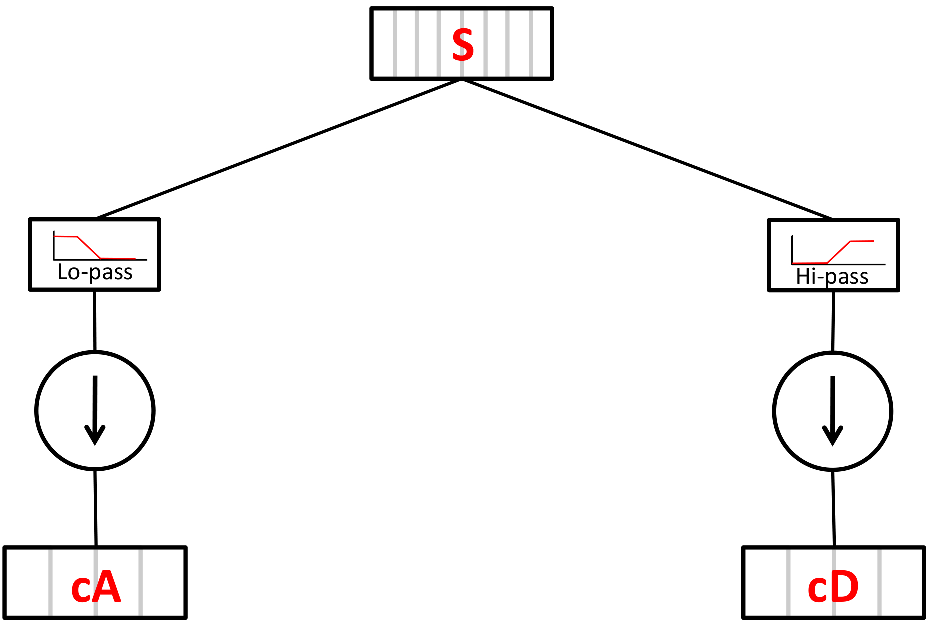
\includegraphics[width=85mm]{LitRev_DWTstep.pdf}
\begin{picture}(0,0)
%\put(-195,133){Scale}
%\put(-22,-7){Time}
\end{picture}
\caption{A single wavelet decomposition step.}
\label{fig:LitRev_DWTstep.pdf}
\end{figure}

%LitRev_DWTtree.pdf
\begin{figure}
\centering
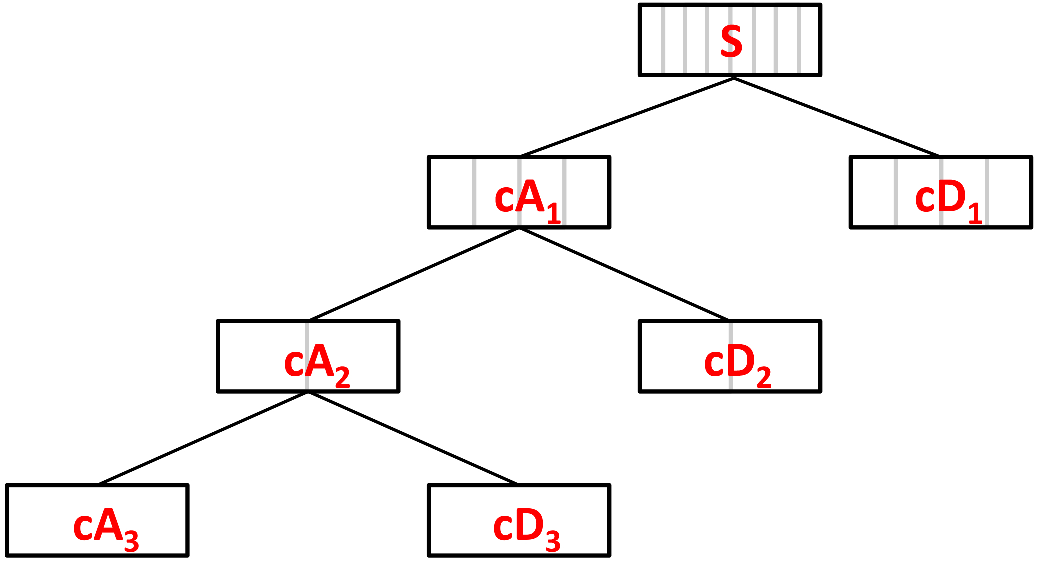
\includegraphics[width=85mm]{LitRev_DWTtree.pdf}
\begin{picture}(0,0)
%\put(-195,133){Scale}
%\put(-22,-7){Time}
\end{picture}
\caption{Three level wavelet decomposition tree.}
\label{fig:LitRev_DWTtree.pdf}
\end{figure}

The multi-resolution properties of the wavelet transform has made the Wavelet transform popular in a range of audio and speech applications where much of the information of interest is located in the lower frequency bands \cite{Sinha1993}\cite{Czyzewski1995}\cite{Lambrou1998}\cite{Biscainho2000}\linebreak[0]\cite{Tzanetakis2001}\linebreak[0]\cite{Zurera2001}\cite{Lin2005}\cite{Nongpiur2008}. Equally the computational efficiency of the discrete wavelet transform is cited \cite{Kadambe1992} as a significant advantage over the \gls{fft} with an $O(N)$ complexity compared to\linebreak[0] $O(N\log{N})$ for the \gls{fft} \cite{Mallat1999}. In \cite{Kadambe1992} the authors report ``superior pitch detection performance'' citing the Wavelet transforms computational efficiency, temporal resolution and its suitability of the pitch periods found in the analysed material. Speech applications in particular report good spectral estimation capabilities \cite{Hu2004}, good de-noising capabilities \cite{Donoho1995}\cite{Seok1997}, and good compression performance \cite{Sinha1993}\cite{Fgee1999}. Several authors propose wavelets used as a basis for audio classification applications \cite{Lambrou1998}\cite{Tzanetakis2001}\cite{Lin2005} and report that a specific advantage of the wavelet basis is its compact representation compared to the time domain signal which decreases processing delay/cost \cite{Lambrou1998}.

An early wavelet based click detection algorithm proposes to detect clicks by analysing the wavelet coefficients of the signal for discontinuities \cite{Czyzewski1995}. The authors apply a neural network algorithm to robustly detect and classify pulses although the authors note that the required training stage is both ``a complex and time-consuming procedure''. While not explicitly discussed the authors appear to be targeting extremely short time pulses of the order of 1 or 2 samples, or what they call ``parazite impulses''.

More recently wavelet bases have been used to detect impulsive noise in speech data by taking advantage of the relatively slow time-varying nature of speech and the Lipschitz regularity of the speech components \cite{Nongpiur2008}. For this application the scope of the corrupted samples appeared larger with suggested possible corruptions including gunshots, rain drops and keyboard typing noise. The author reported that the algorithm managed to reduce the rain drop noise in an instantaneous mixture of speech and rain noise. It was noted that this was the only noise application demonstrated and that it was never intended to completely remove the noise entirely. It was also noted that additional noise suppression algorithms seem to have been used as well as a speech enhancement algorithm. The extent to which this algorithm would reduce the nuisance of longer and louder pulses was not explored, but would have been interesting.

\subsubsection{Wavelet Packet Transform (WPT)}
The \gls{wpt} can be seen as a generalisation of the Wavelet transform in that it extends the link between multi-resolution approximations and wavelets. The \gls{wpt} can also be seen as a natural extension of \gls{mtse} \cite{Thomson1982}. While the \gls{dwt} decomposes only the approximation coefficients the \gls{wpt} applies the decomposition step symmetrically throughout the tree as seen in Figure~\ref{fig:LitRev_WPTtree.pdf}. Since the standard \gls{dwt} algorithm is limited to wavelet bases that increase by a power of two towards the higher scales (low frequencies) it is possible that some other combination of bases could provide a better basis in some applications \cite{Coifman1992a}.

%LitRev_WPTtree.pdf
\begin{figure}
\centering
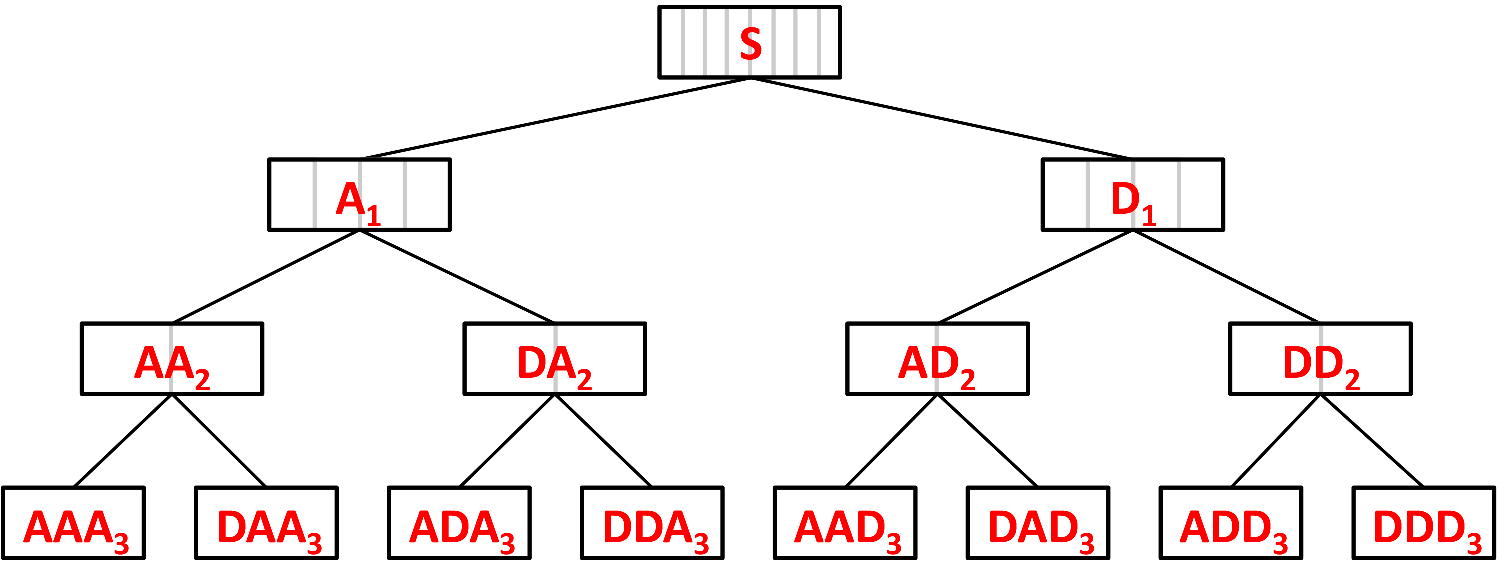
\includegraphics[width=125mm]{LitRev_WPTtree.pdf}
\begin{picture}(0,0)
%\put(-195,133){Scale}
%\put(-22,-7){Time}
\end{picture}
\caption{Three level wavelet packet decomposition tree.}
\label{fig:LitRev_WPTtree.pdf}
\end{figure}

In a recent study comparing the \gls{wpt} to other spectrum estimation techniques it was generally found that the \gls{wpt} ``operated well for all types of sources and its performances were comparable or at times even better than other existing \linebreak[0]approaches.''\linebreak[2]\cite{Ariananda2013}. In particular it was found that \gls{wpt} performed well in reducing variance in the stop bands.

The authors of \cite{He2008} developed a psychoacoustic model based around the \gls{wpt} and found that not only was the \gls{wpt} computationally more efficient than a Fourier transform-based alternative but it also provided a better spectral resolution. For psychoacoustic applications it was found that the generalization of the \gls{dwt} yielded a better approximation of the critical bands employed \cite{Carnero1999}\cite{He2008} compared to similar \gls{dwt} based models \cite{Sinha1993}\cite{Zurera2001}.

\section{Restoration}\label{sec:LitRev_Restoration}
The restoration of corrupted speech and audio samples by a localised degradation, also referred to as clicks or noise pulses, has inspired much research and many approaches. Corruptions can generally be seen to have varying severity. Clicks and pulses have traditionally been treated as completely corrupted or essentially missing samples transforming the restoration task into one of interpolation of missing samples \cite{Tukey1974}\cite{Tukey1977}\cite{Godsill1998book}.

An exhaustive review of the methods employed in the field up until the year of publishing in 1992 can be found in \cite{Veldhuis1992}. A summary of relevant methods and more recent methods are provided in this section. While the focus of this thesis is the interpolation of audio segments, as with the detection task, some methods or related approaches can be found in the field of image restoration of localised corruptions or other 1 and 2 dimensional implementations.

\subsection{Nonlinear approaches}\label{sec:LitRev_RestorationNonLin}
As noted in section~\ref{sec:LitRevDetMedianFilts}, a classic pulse detection approach in both audio and image processing has been by median filtering. Equally, many of the approaches mentioned previously employ median based approaches for restoring the detected pulses \cite{Tukey1974}\cite{Lee1985}\cite{Heinonen1985}\cite{Heinonen1987}\cite{Maekivirta1991}\cite{Kasparis1993}\cite{Alajlan2004}. In \cite{Bovik1983} it was shown that the optimal order statistics filter (OSF) tends towards a median filter as the noise becomes increasingly impulsive. In particular the median filter is effective when the pulse length is less than half the median window size \cite{Alajlan2004}.

Much of the early work on nonlinear digital smoothing followed the original proposed algorithm by Tukey \cite{Tukey1974}. Following this publication the algorithm, in combination with linear filtering, was applied to speech signals and was found to perform reasonably \cite{Rabiner1975}. The authors noted that the median filter alone, although successful in the preservation of sharp discontinuities not associated with noise, failed to provide sufficient smoothing and was therefore paired with a simple 3-point linear filter. In addition the authors described a double smoothing algorithm which attempted to isolate noisy segments and re-subtract them.


%Median filtering for restoration:
%JAYNAT, N.S.: ‘Average and median based smoothing for improving
%digital speech quality in the presence of transmission errors’,
%IEEE Trans., COM-24,1976, pp. 1043-1045
% \cite{Jayant1976}
%
% ^ Efficacy of employing some simple waveform smoothing. Transmission errors.
%
A similar early approach used to combat the effects of transmission errors in digital speech signals employed simple waveform-smoothing techniques and reported a ``cleaner-sounding'' speech in the presence of ``fairly significant'' error rates \cite{Jayant1976}. The result of this was unfortunately also a smearing of the speech component but the authors found that for high probability of errors this pulse-squelching operation was still perceptually desirable in spite of speech smearing. These results were backed up by a six person subjective study.

%\todo{Add this reference in!}
%RABINER, L.R., SAMBUR, M.R., and SCHMIDT, C.Es
%of a nonlinear smoothing algorithm to speech processing.
%IEEE Trans., ASSP-32, (3), 1975
% \cite{Rabiner1975}
%
% ^ Median and linear smoothing combined.
%   Linear smoothing is rarely enough.
%
% "Generalized median filtering and related nonlinear filtering techniques"
% Another median+linear smoother

These methods all appear to have been applied indiscriminately to the data sequences which bore a cost to the signal fidelity.

%Median LPC hybrid
%NIEMINEN, HEINONEN, P., and NEUVO, Y.: ‘Suppression
%and detection of impulsive type interference using adaptive median
%hybrid filter’. IEEE Proc. ICASSP 1987, pp. 117-120.

Realising the power of both linear and non-linear approaches to non-stationary noise detection and restoration, a range of \emph{hybrid} approaches arose \cite{Nieminen1987a}\cite{Lee1985}\cite{Heinonen1987}. A \gls{mtm} filter, was found to outperform a standard median filter in the task of preserving naturally sharp edged in signals \cite{Lee1985}. The \gls{mtm} filter quite simply replaces values of a frame with the average of a subframe selected around the outer frame's median value \cite{Lee1985}. An \gls{fmh} filter was designed with the aim of outperforming the standard median filter computationally. The \gls{fmh} filter was found to perform similarly the standard median filter \cite{Heinonen1987}. Lastly the \gls{amh} filters, proposed in \cite{Nieminen1987a}, employ multiple substructures which was considered ``ideal for processing of signals with statistics which change abruptly''. The theory is that at least one of the substructures will have adapted to a local change in the signal characteristics, whereas short non-stationary changes will be omitted. For the examples presented, this approach conserved sharp local changes while a comparable \gls{lms} filter did not \cite{Nieminen1987a}.

From a computational perspective, median filters involve a sequence of searching and sorting steps and despite dedicated hardware for these operations these procedures are generally computationally intensive \cite{Kundu1984}. A generalised mean implementation for black and white photos showed similar, and in some cases better, performance to the median filter while maintaining a distinct computational advantage \cite{Kundu1984}.

%Lee: L and M filters + useful modification: MTM filter
% "combine properties of both the linear and median filters"
% "The concept of double-window filtering is introduced as a refinement of MTM filtering"
% "It was observed that M filters offers a more favorable combination of the characteristics of running mean and median filters than the L filters"
% "The MTM filters were shown to provide better overall characteristics. In fact, we have seen that MTM filters can preserve noisy edges better than can median filters."

%Heinonen: \gls{fir}-median hybrid (FMH) filters (M filter)
% "The \gls{fir}-median Hybrid (FMH) filters require significantly less computations than the Standard Median (SM) filters.

%Nieminen: Adaptive Median Hybrid (AMH) filters
% "In the AMH filters, adaptive filter substructures are used
% to estimate the current signal value from the future and
% past signal values. The output of the overall filter is the
% median of the %adaptive filter outputs and the currents ignal
% value. This kind of nonlinear filter structure is shown to
% adapt and preserve rapid changes in signal characteristics
% well. However, it filters out short duration interferences. By
% examining the difference between the original and filtered
% data, interferences can be detected."

% Non-linear, minimum or maximum of neighborhood based on dark or bright spot. (Alajlan based on Windyga, good explanation of Windyga in Alajlan)
In the field of image processing the median filter is still an integral part in most state-of-the-art impulsive noise filters \cite{Alajlan2004}. Other popular non-linear methods employed have been the maximum-minimum method \cite{Xu1998}, the peak-and-valley filter\linebreak[2]\cite{Windyga2001} and a modified maximum-minimum approach \cite{Alajlan2004} which aims to apply a maximum-minimum approach to selected samples only. All these non-linear approaches were found to have similar performance but with the median filter bearing a higher computational cost \cite{Alajlan2004}.

% waveform substitution schemes
% \cite{Goodman1986}\cite{Wasem1988}\cite{Niediwiecki2001}
A more direct and heuristic approach to waveform and audio restoration of longer gaps is found in waveform substitution \cite{Goodman1986} or ``smart copying'' \cite{Niediwiecki2001}. An audio segment immediately prior to a corruption is used as a template for finding matches earlier in the sequence. It is assumed that what follows the best match for the template will be a good substitute for the corrupted segment. Given that speech signals ``display quasi-stationary intervals'' \cite{Goodman1986} this algorithm produces feasible looking results if the corruption does not straddle regions with high-energy voiced speed, low-level unvoiced speech or silence \cite{Goodman1986}. Waveform substitution has been confirmed through several objective listening tests to have ``satisfactory'' results \cite{Niediwiecki2001}. In addition the method excels by being computationally simple \cite{Niediwiecki2001}.

%pitch detection
An extension of the basic waveform substitution algorithm, an additional pitch detection extension, was proposed. If a pitch estimate is available, the pitch period prior to the corruption may be reproduced throughout the corruption \cite{Goodman1986}. No direct results were presented to quantify the performance of this addition but a later publication ranks a pitch waveform replication algorithm as producing the highest quality results based on subjective tests \cite{Wasem1988}. In the tests performed in \cite{Wasem1988}, the method was compared with a simple silence insertion and packet repetition algorithms suffering from obviously audible discontinuities \cite{Goodman1986} in addition to one and two-sided waveform substitution algorithms \cite{Goodman1986}. It was noted that while the pitch waveform replicator produced the highest quality results it was not the most computationally complex nor did it produce the longest delays of the tested algorithms \cite{Wasem1988}.

A similar heuristic pitch based approach proposes to model speech as a series of spectral peak tracks that are ``born'' and ``die'' employing the \gls{stft} \cite{Maher1994}. First proposed by \cite{McAulay1986} this method has since been referred to as MQ representation (after the authors' names) and been applied to the task of speech interpolation \cite{Maher1994}. Many other authors have applied sinusoidal models for speech modeling in a variety of applications \cite{Godsill1998book}\cite{Vera-Candeas2003}\cite{Wells2006} which attempts in some cases to generalise the glottal excitation model in speech \cite{McAulay1986}.
%other sinusoidal based approaches

% P. A. A. Esquef, L. W. P. Biscainho, V. Välimäki, and M. Karjalainen, "Removal of Long Pulses from Audio Signals Using Two-pass Split-Window Filtering", presented at the 112th AES Convention, preprint no. 5535, Munich, Germany, May 10-13, 2002. \cite{Esquef2002a}

\subsection{Linear approaches}\label{sec:LitRev_RestorationLin}
%Skip
% Band limited extrapolation/band-limited interpolation
% \cite{Papoulis1975}\cite{Ferreira2001}

In speech signals a popular and successful method of interpolation is the \gls{ar} approach \cite{Vaseghi1988thesis}\cite{Godsill1998book}\cite{Kauppinen2002b}. An early approach using it demonstrated that this method produced satisfactory results for speech signals particularly, based on both objective and subjective results, and furthermore established the feasibility of real-time implementation of such methods \cite{Janssen1986}. Independent development applied the methods to audio restoration applications \cite{Vaseghi1988thesis}\cite{Vaseghi1990}.

Typically longer stretches of audio interpolation have been difficult applications for \gls{ar} models \cite{Veldhuis1992}\cite{Kauppinen2002b}, but modified \gls{ar} based models have been applied to the pure extrapolation problem with some success on longer gaps \cite{Kauppinen2002b}. The basic \gls{ar} models, and later least squares \gls{ar} extensions \cite{Godsill1998book}, have also been paired with synthesis filters designed to excite the \gls{ar} model to achieve longer gap extrapolation with lower model orders \cite{Esquef2006}. This method achieves comparable perceptual quality to higher order \gls{ar} models given significantly lower model complexity \cite{Esquef2006}.

In general many authors have considered \gls{lpc} and \gls{ar} models for audio and speech data \cite{Vaseghi1990}\cite{Czyzewski1995}\cite{Godsill1998}. A more comprehensive review of \gls{ar}, \gls{lpc} and warped-based methods were covered in section~\ref{sec:LitRevAR} from the perspective of modeling speech and audio in the detection application.

%An Efficient Model-Based Method for Reconstruction of Audio Signals Across Long Gaps
% \cite{Esquef2006} (based on \cite{Kauppinen2002a} and \cite{Kauppinen2002b})
% The use of a maximally-decimated filterbank renders easier
%the interpolation task within a subband. This is due to the decreased
%number of resonance modes to be modeled, allowing
%model order reduction. In addition, the length of the gap to fill
%in shortens by the decimation factor of the subband. For the two
%lowest subbands this factor is 1/32.
%
%In such situations  \gls{ar} based interpolators tend to perform poorly toward the middle of the gap, where the energy of the
%interpolated signal decreases [13].
%The aforementioned signal energy reduction occurs in part
%due to the minimization of the \gls{ar} modeling error, which is employed
%to solve for the unknown samples within a given gap
%[15]. In the ideal case of a null modeling error, the resulting interpolated
%signal would be determined mainly by the impulse
%response of the \gls{ar} model.%


% \cite{Vaseghi1990}: LPC. "An interpolation algorithm was
%described that takes advantage of the quasi-periodic
%nature of glottal excitation and provides better estimates
%than the existing method."

% interpolators based on sinusoidal modeling
% \cite{Maher1994}\cite{Godsill1998book}

% subband methods
% \cite{Montresor1991} \cite{Cocchi2001}

%Low frequency pulse corruption:
%|P. A. A. Esquef, L. W. P. Biscainho, and V. Välimäki, "An Efficient Algorithm for the Restoration of Audio Signals Corrupted with Low-Frequency Pulses", Journal of the Audio Engineering Society, vol. 51, no. 6, pp. 502-517, June 2003
% \cite{Esquef2003a}

%Wavelet Shrinkage:
%|L. W. P. Biscainho, F. P. Freeland, P. A. A. Esquef, and P. S. R. Diniz, "Wavelet Shrinkage De-noising Applied to Real Audio Signals under Perceptual Evaluation," in Proc. X European Signal Processing Conf. (EUSIPCO 2000), pp. 2061-2064, Tampere, Finland, September 2000.
% \cite{Biscainho2000}

%

%\subsection{Median filtering}

% \cite{Nongpiur2008} : "On the basis of these differences, an algorithm was developed
%to identify and suppress wavelet coefficients that correspond to
%impulse noise."

% A comprehensive review of restoration methods can be found in \cite{Veldhuis1992}

%\section{Residual Restoration}
%A variety of restoration algorithms have been tested for the restoration of the residual audio component. Based on the nature of the detection algorithm, the restoration step can be done either on the wavelet coefficients or on the time series data.

%\todo{something more}

\section{Keyboard detection and removal systems}
For the keystroke removal application a couple of articles have suggested similar systems \cite{Subramanya2007}\cite{Sugiyama2007}\cite{Abramson2007}\cite{Sugiyama2013}. 

\cite{Subramanya2007} proposes the \gls{ukd} algorithm. This algorithm relies on \gls{stft} and exploits the assumption of smoothness in the spectral coefficients during normal speech. Using an \gls{ar} filter on each frequency band the filtering error is considered as a joint probability and thresholded to expose detections. This method is described in great detail in equations \ref{eq:Subramanya2007} and \ref{eq:Subramanya2007_2}. The implementation presented by the authors rely on a lookahead of 2 buffers (of 20 ms) to make their detection requiring additional latency in a potential communication network. Additionally the authors propose to increase the robustness of their system by implementing a constrained detection step using the \gls{os} to feed information back to the algorithm to verify if the detection was in fact correct or not. The approach taken by the authors to restore corrupted coefficients is to replace them with new estimates using a \gls{map} based approach \cite{Raj2004}. The authors assumes the spectral coefficients are modeled as a stationary Gaussian process with a mean and variance. These statistical parameters are learned on an uncorrupted sequence. The method estimates the \gls{map} estimate of the the log-magnitude of the coefficients rather than the coefficients themselves. Further, the authors propose to improve these reconstructions by imposing constraints on the statistical parameters.
The method proposed in \cite{Subramanya2007} relies on 40 ms lookahead, trained parameters for the speech reconstruction algorithm and, in the case of \gls{ekd} \gls{os} information about keyboard inputs. These elements make the algorithm unsuitable for real-time implementation.


and \cite{Sugiyama2007} propose algorithms specifically for the keyboard stroke detection and removal application. All of these methods rely on the \gls{stft} as a basis for detection using features such as the shape and change of the power spectrum \cite{Sugiyama2007}, \gls{ar} estimation error \cite{Subramanya2007}\cite{Kauppinen2002} or a Bayesian speech estimator \cite{Abramson2007}. In \cite{Godsill1998book} various \gls{ar} based detection methods are proposed and it was found that pairing the \gls{ar} model with a basis, e.g. a sinusoid, gives a generally applicable approach with improved performance. In \cite{Vaseghi1990} the authors find that \gls{ar} processes are ``adequate for modelling of speech signals whereas they can not model impulsive disturbances.''.

\section{Chapter summary}
This chapter has aimed to summarise the relevant literature associated with the applications, techniques and theory presented throughout this thesis.

A range of applications have previously been proposed for the \gls{apr} application which all utilise multiple microphones to implement a touchscreen interface \cite{US8174547}\linebreak[0]\cite{US8233353}\linebreak[0]\cite{TouchSystems2006}\cite{US7411581}\cite{WO2006108443}. While a few different approaches are taken the functional elements of these methods all rely on there being multiple sources.

In \cite{Burke2013} a survey of factorisation methods found \gls{pca} to be an effective approach to feature extraction for classification applications, and in \cite{Tipping1999} \gls{pca} was put into a probabilistic framework with \gls{ppca}.

%For the keystroke removal application a couple of articles have suggested similar systems \cite{Subramanya2007}\cite{Sugiyama2007}\cite{Abramson2007}. \cite{Subramanya2007} and \cite{Sugiyama2007} propose algorithms specifically for the keyboard stroke detection and removal application. All of these methods rely on the \gls{stft} as a basis for detection using features such as the shape and change of the power spectrum \cite{Sugiyama2007}, \gls{ar} estimation error \cite{Subramanya2007}\cite{Kauppinen2002} or a Bayesian speech estimator \cite{Abramson2007}. In \cite{Godsill1998book} various \gls{ar} based detection methods are proposed and it was found that pairing the \gls{ar} model with a basis, e.g. a sinusoid, gives a generally applicable approach with improved performance. In \cite{Vaseghi1990} the authors find that \gls{ar} processes are ``adequate for modelling of speech signals whereas they can not model impulsive disturbances.''.

Restoration approaches applicable to longer gaps ranged from heuristic waveform substitution methods \cite{Goodman1986}\cite{Niediwiecki2001}, pitch based methods modeling speech as spectral peak tracks \cite{Maher1994}\cite{McAulay1986} to \gls{ar} interpolators \cite{Esquef2006} based on a least squares adaption of the \gls{ar} process \cite{Godsill1998book}.
%synthesis filters designed to excite the \gls{ar} model to achieve longer gap extrapolation with lower model orders \cite{Esquef2006}



% ------------------------------------------------------------------------


%%% Local Variables:
%%% mode: latex
%%% TeX-master: "../thesis"
%%% End:



